\section{Getting Started}
\label{sec:getting-started}

\subsection{Installation}
\label{sec:installation}

\subsubsection{Setup}
\label{sec:setup}

\begin{itemize}
\item Before installing the Event-B XText Front-end feature, you need to add the XText update site (\url{http://download.eclipse.org/modeling/tmf/xtext/updates/composite/releases/}) as an additional software site (see Figure~\ref{fig:xtext-updatesite}).
\begin{figure}[!htbp]
  \centering
  \ifplastex
  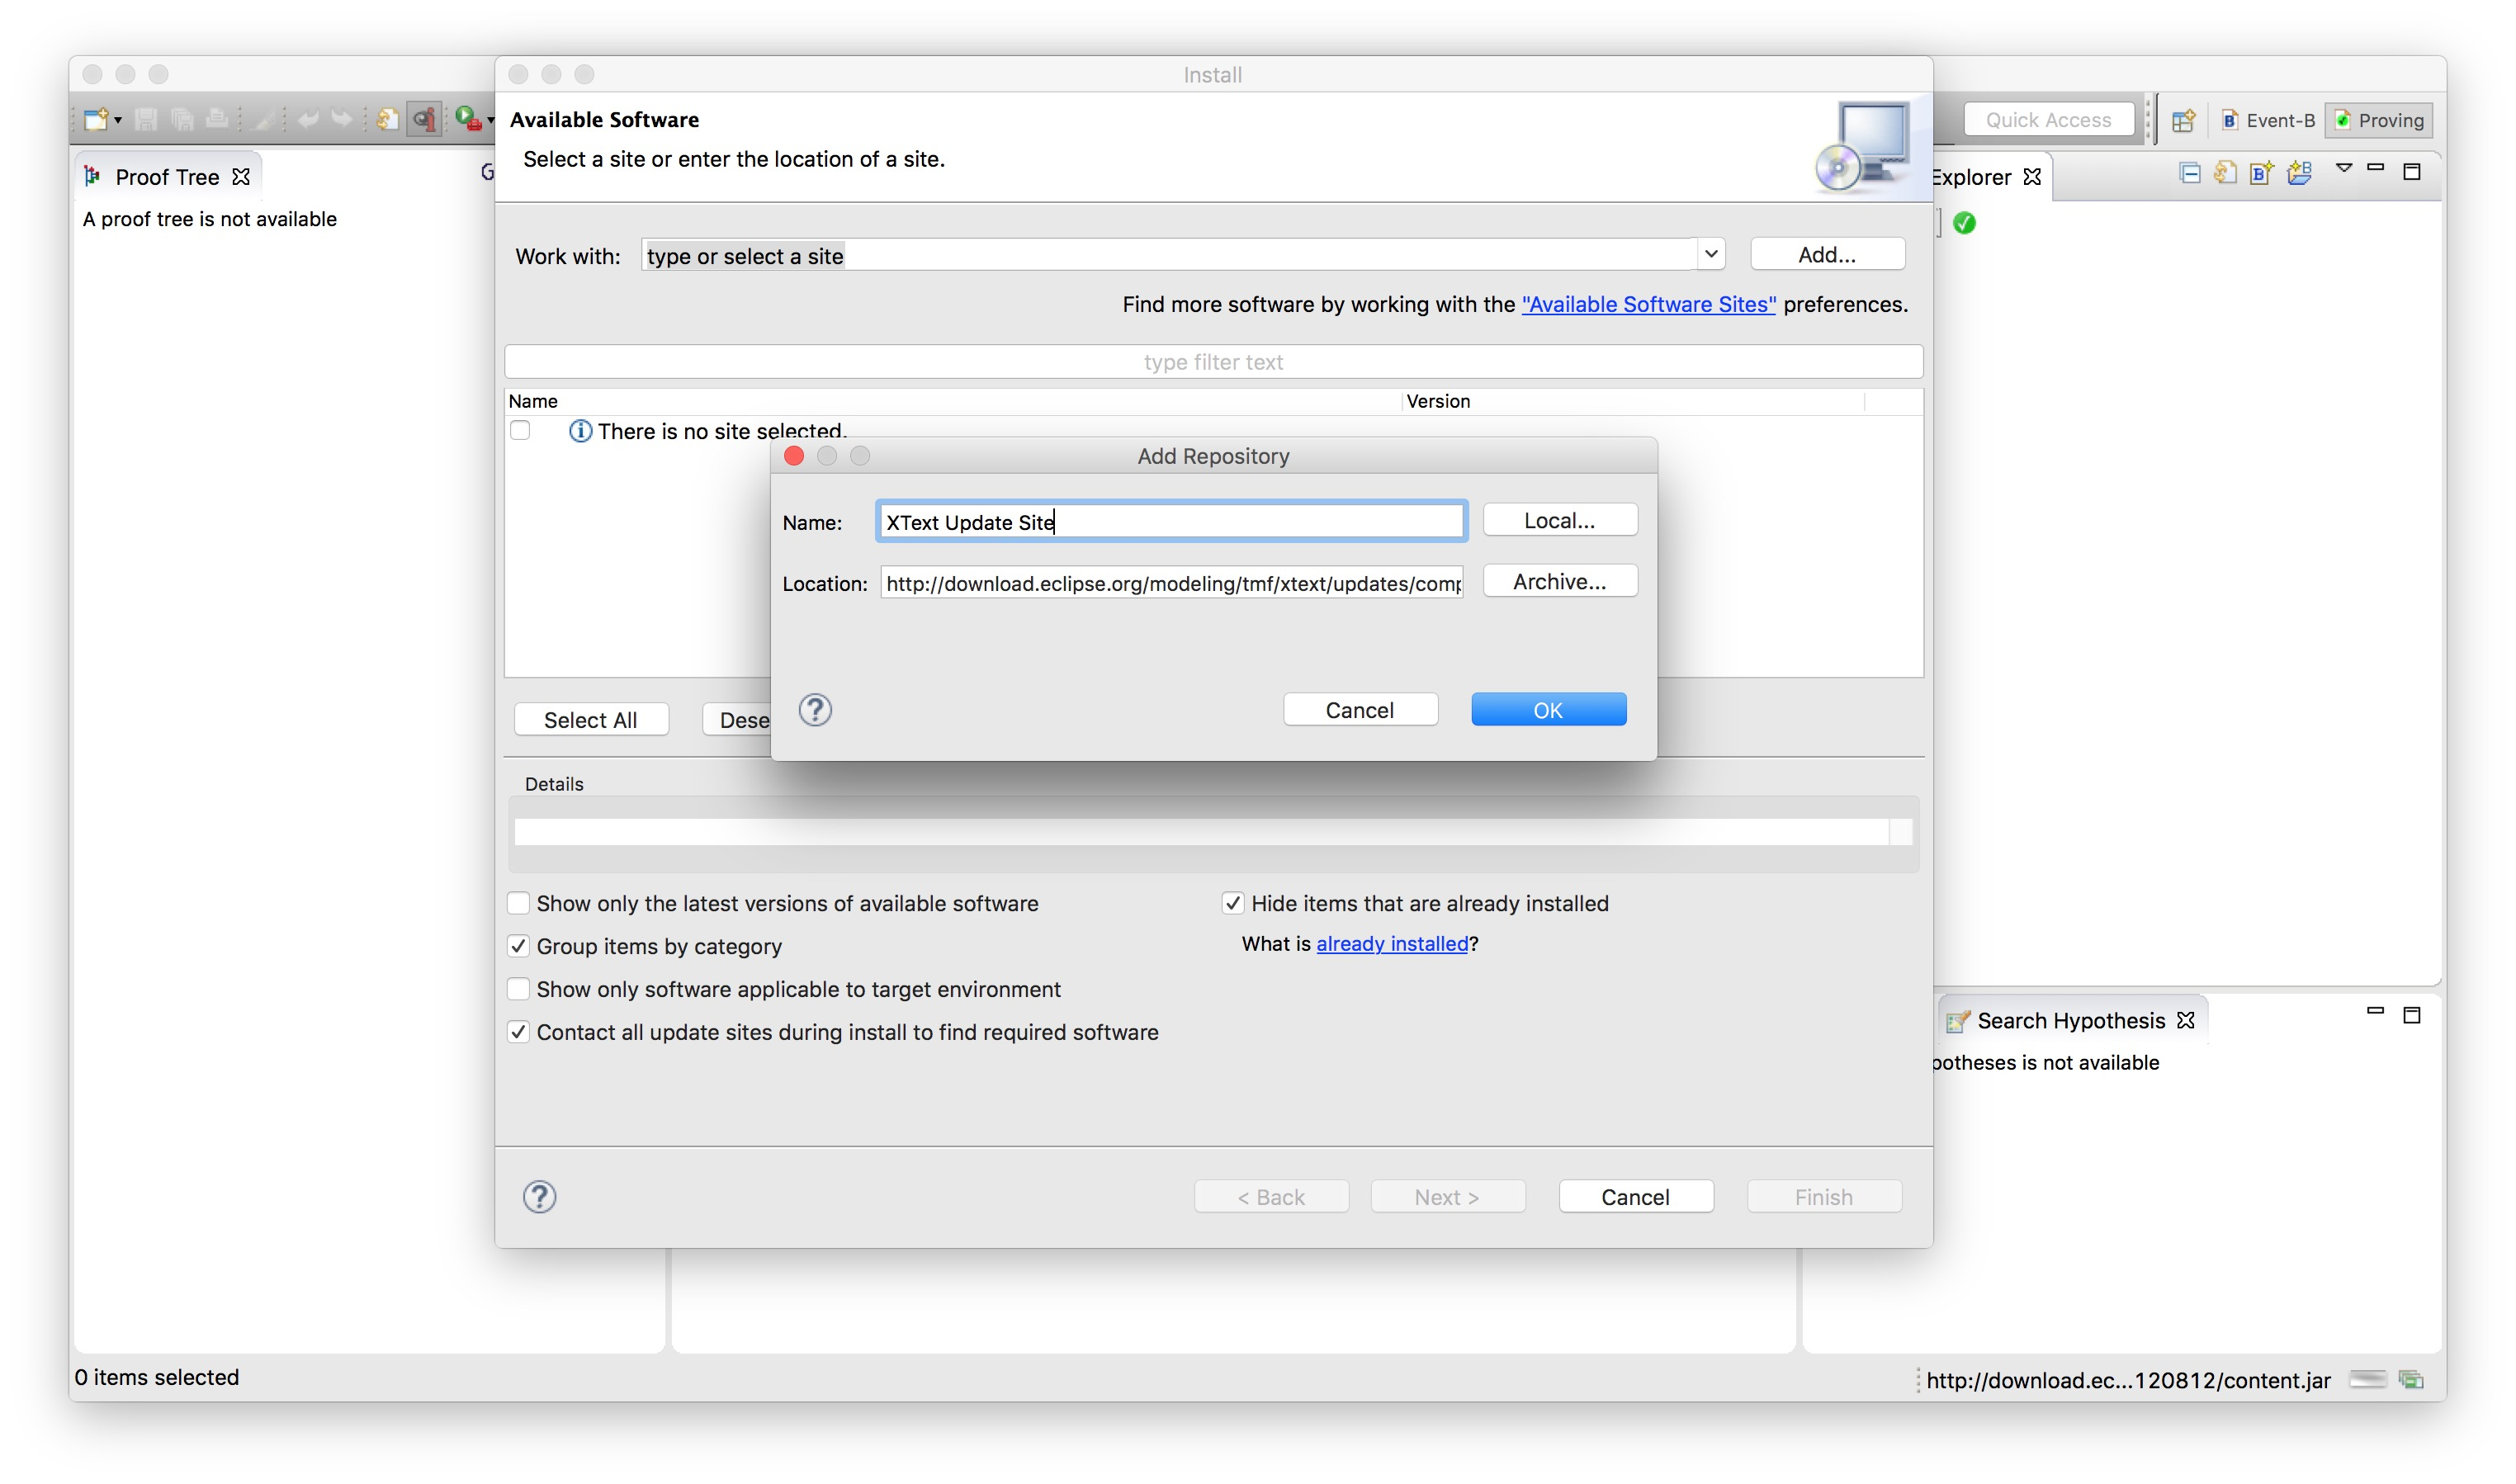
\includegraphics[width=512]{figures/XTextUpdateSite}
  \else
  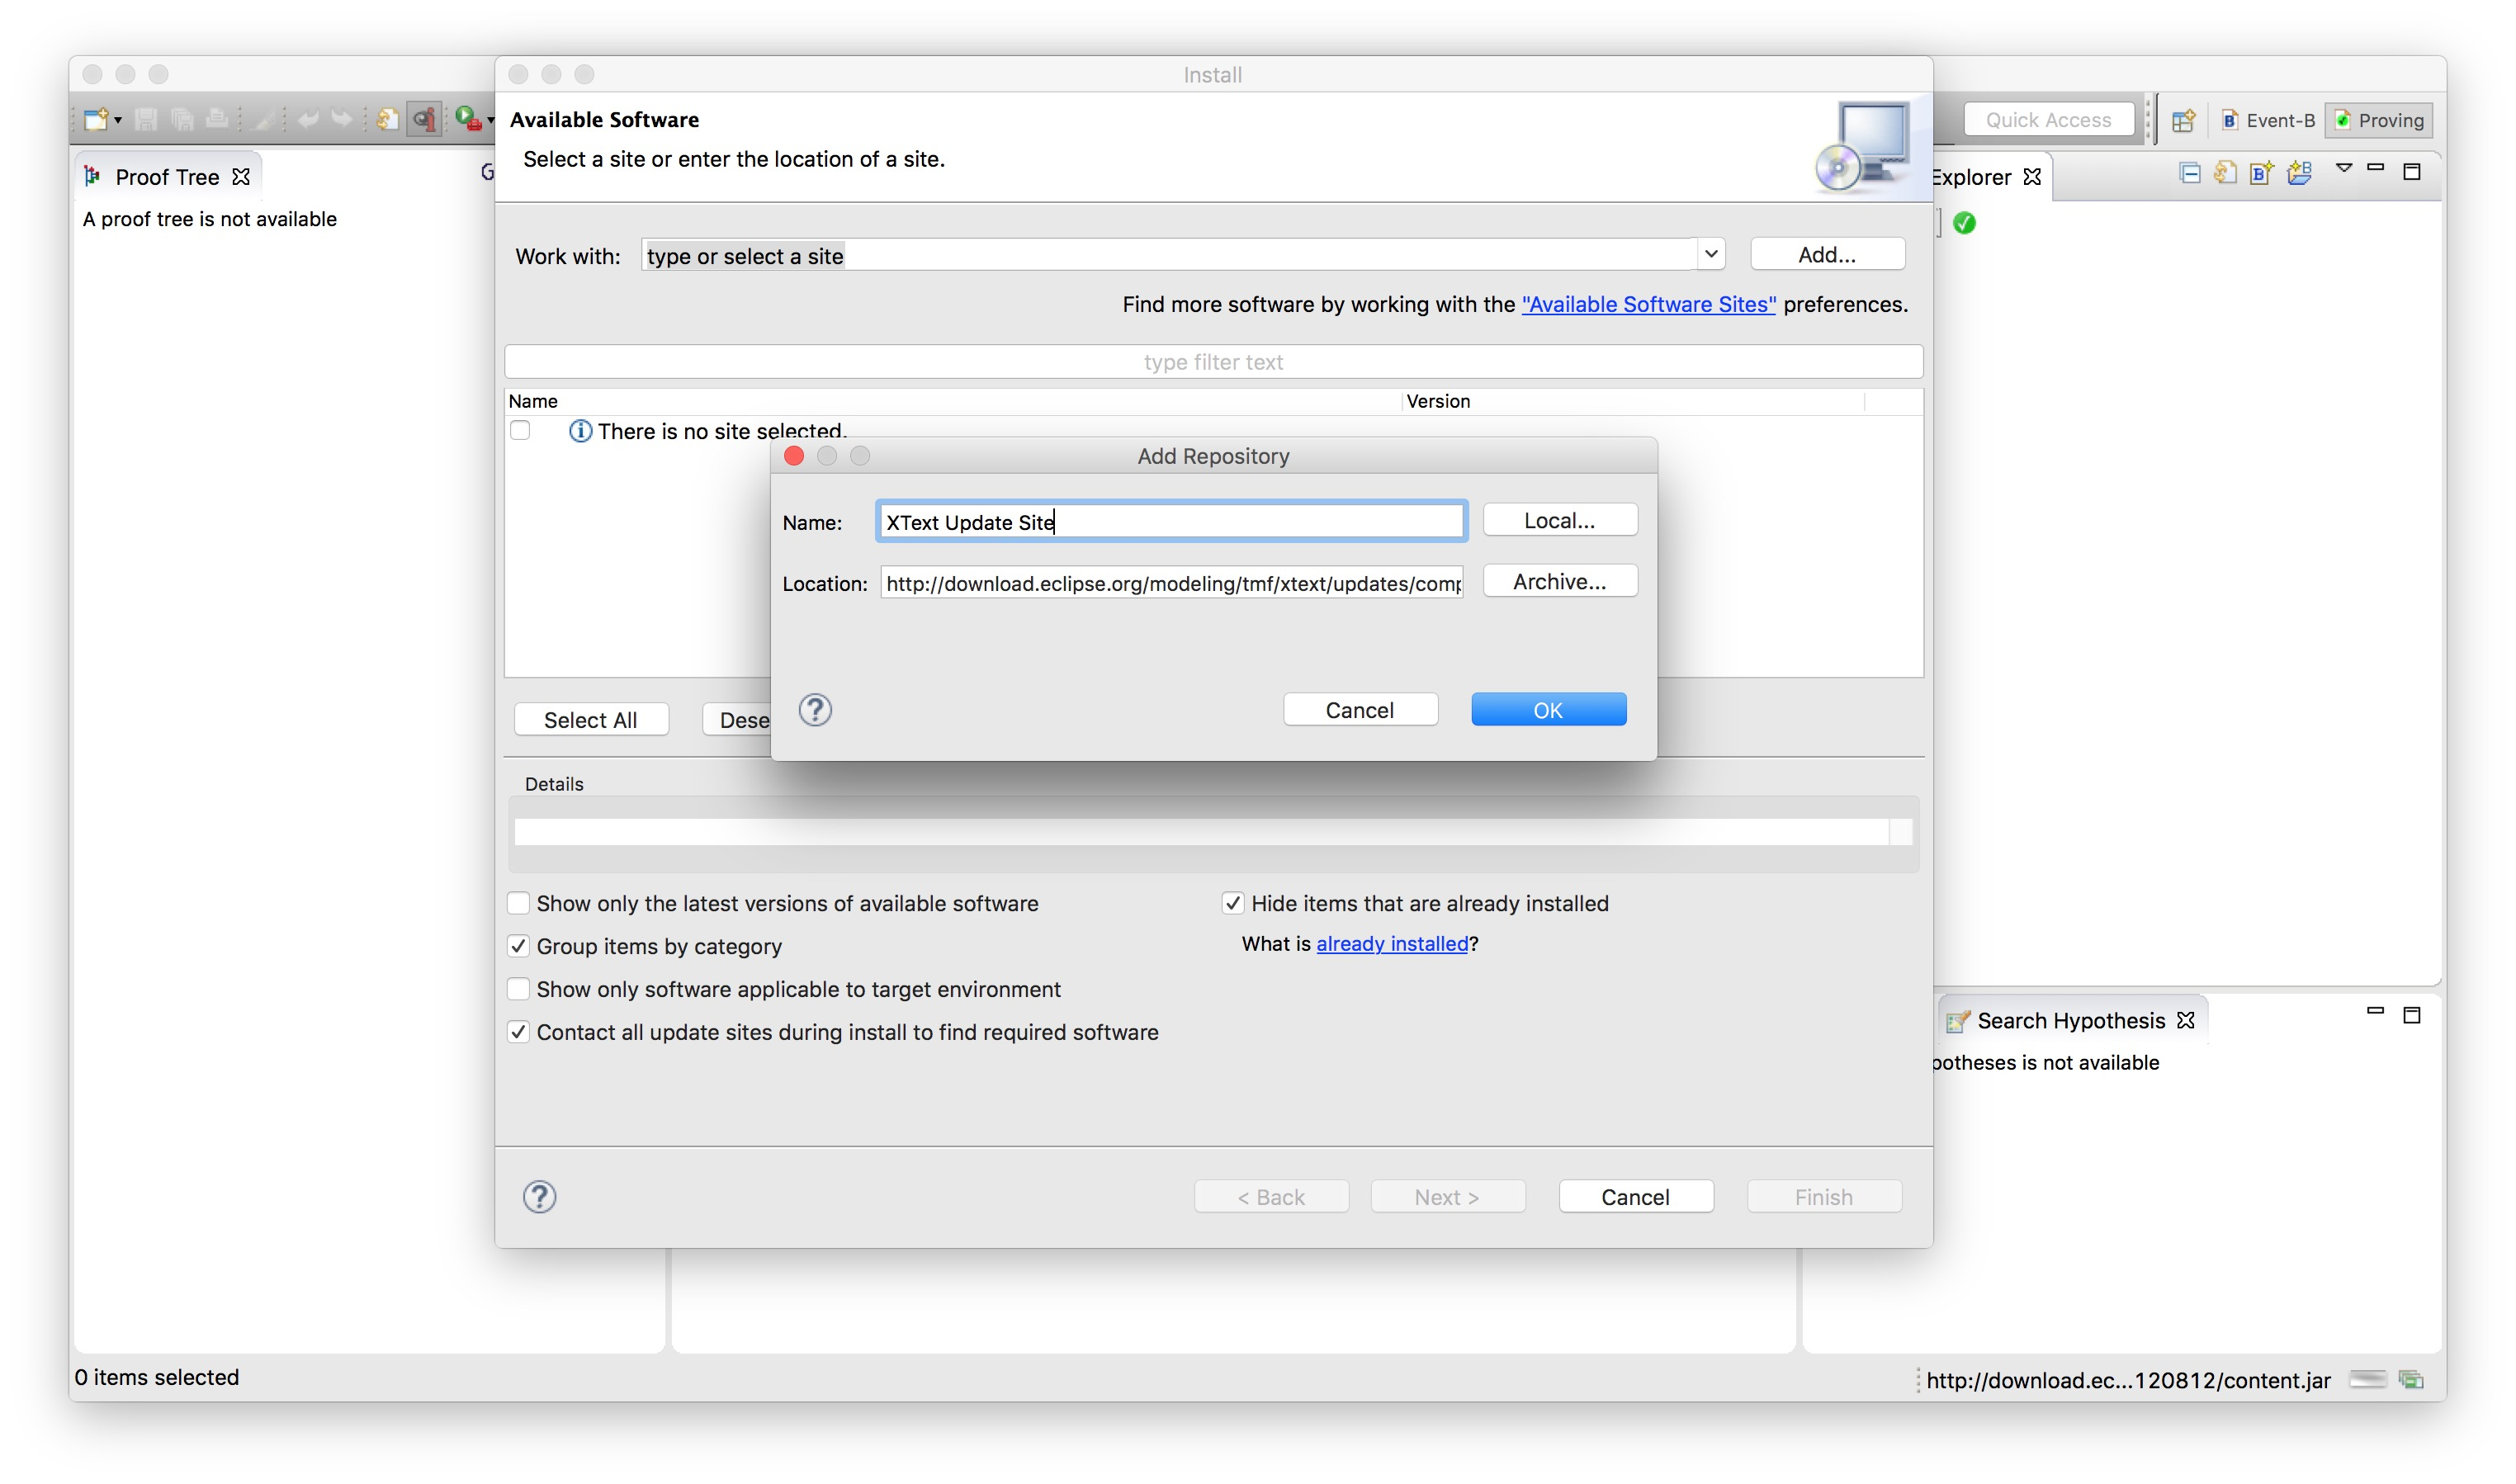
\includegraphics[width=0.9\textwidth]{figures/XTextUpdateSite}
  \fi
  \caption{Adding XText Update Site}
  \label{fig:xtext-updatesite}
\end{figure}


\item The Event-B XText front-end feature is available from the main Rodin update site (under ``Editors'' category). There are two versions of the feature, \emph{Event-B XText} providing facilities for working with Event-B XText Front-end, and the \emph{Event-B XText (SDK)} is the feature including source code for software developers (see Figure~\ref{fig:EventBXText-installation}).
\begin{figure}[!htbp]
  \centering
  \ifplastex
  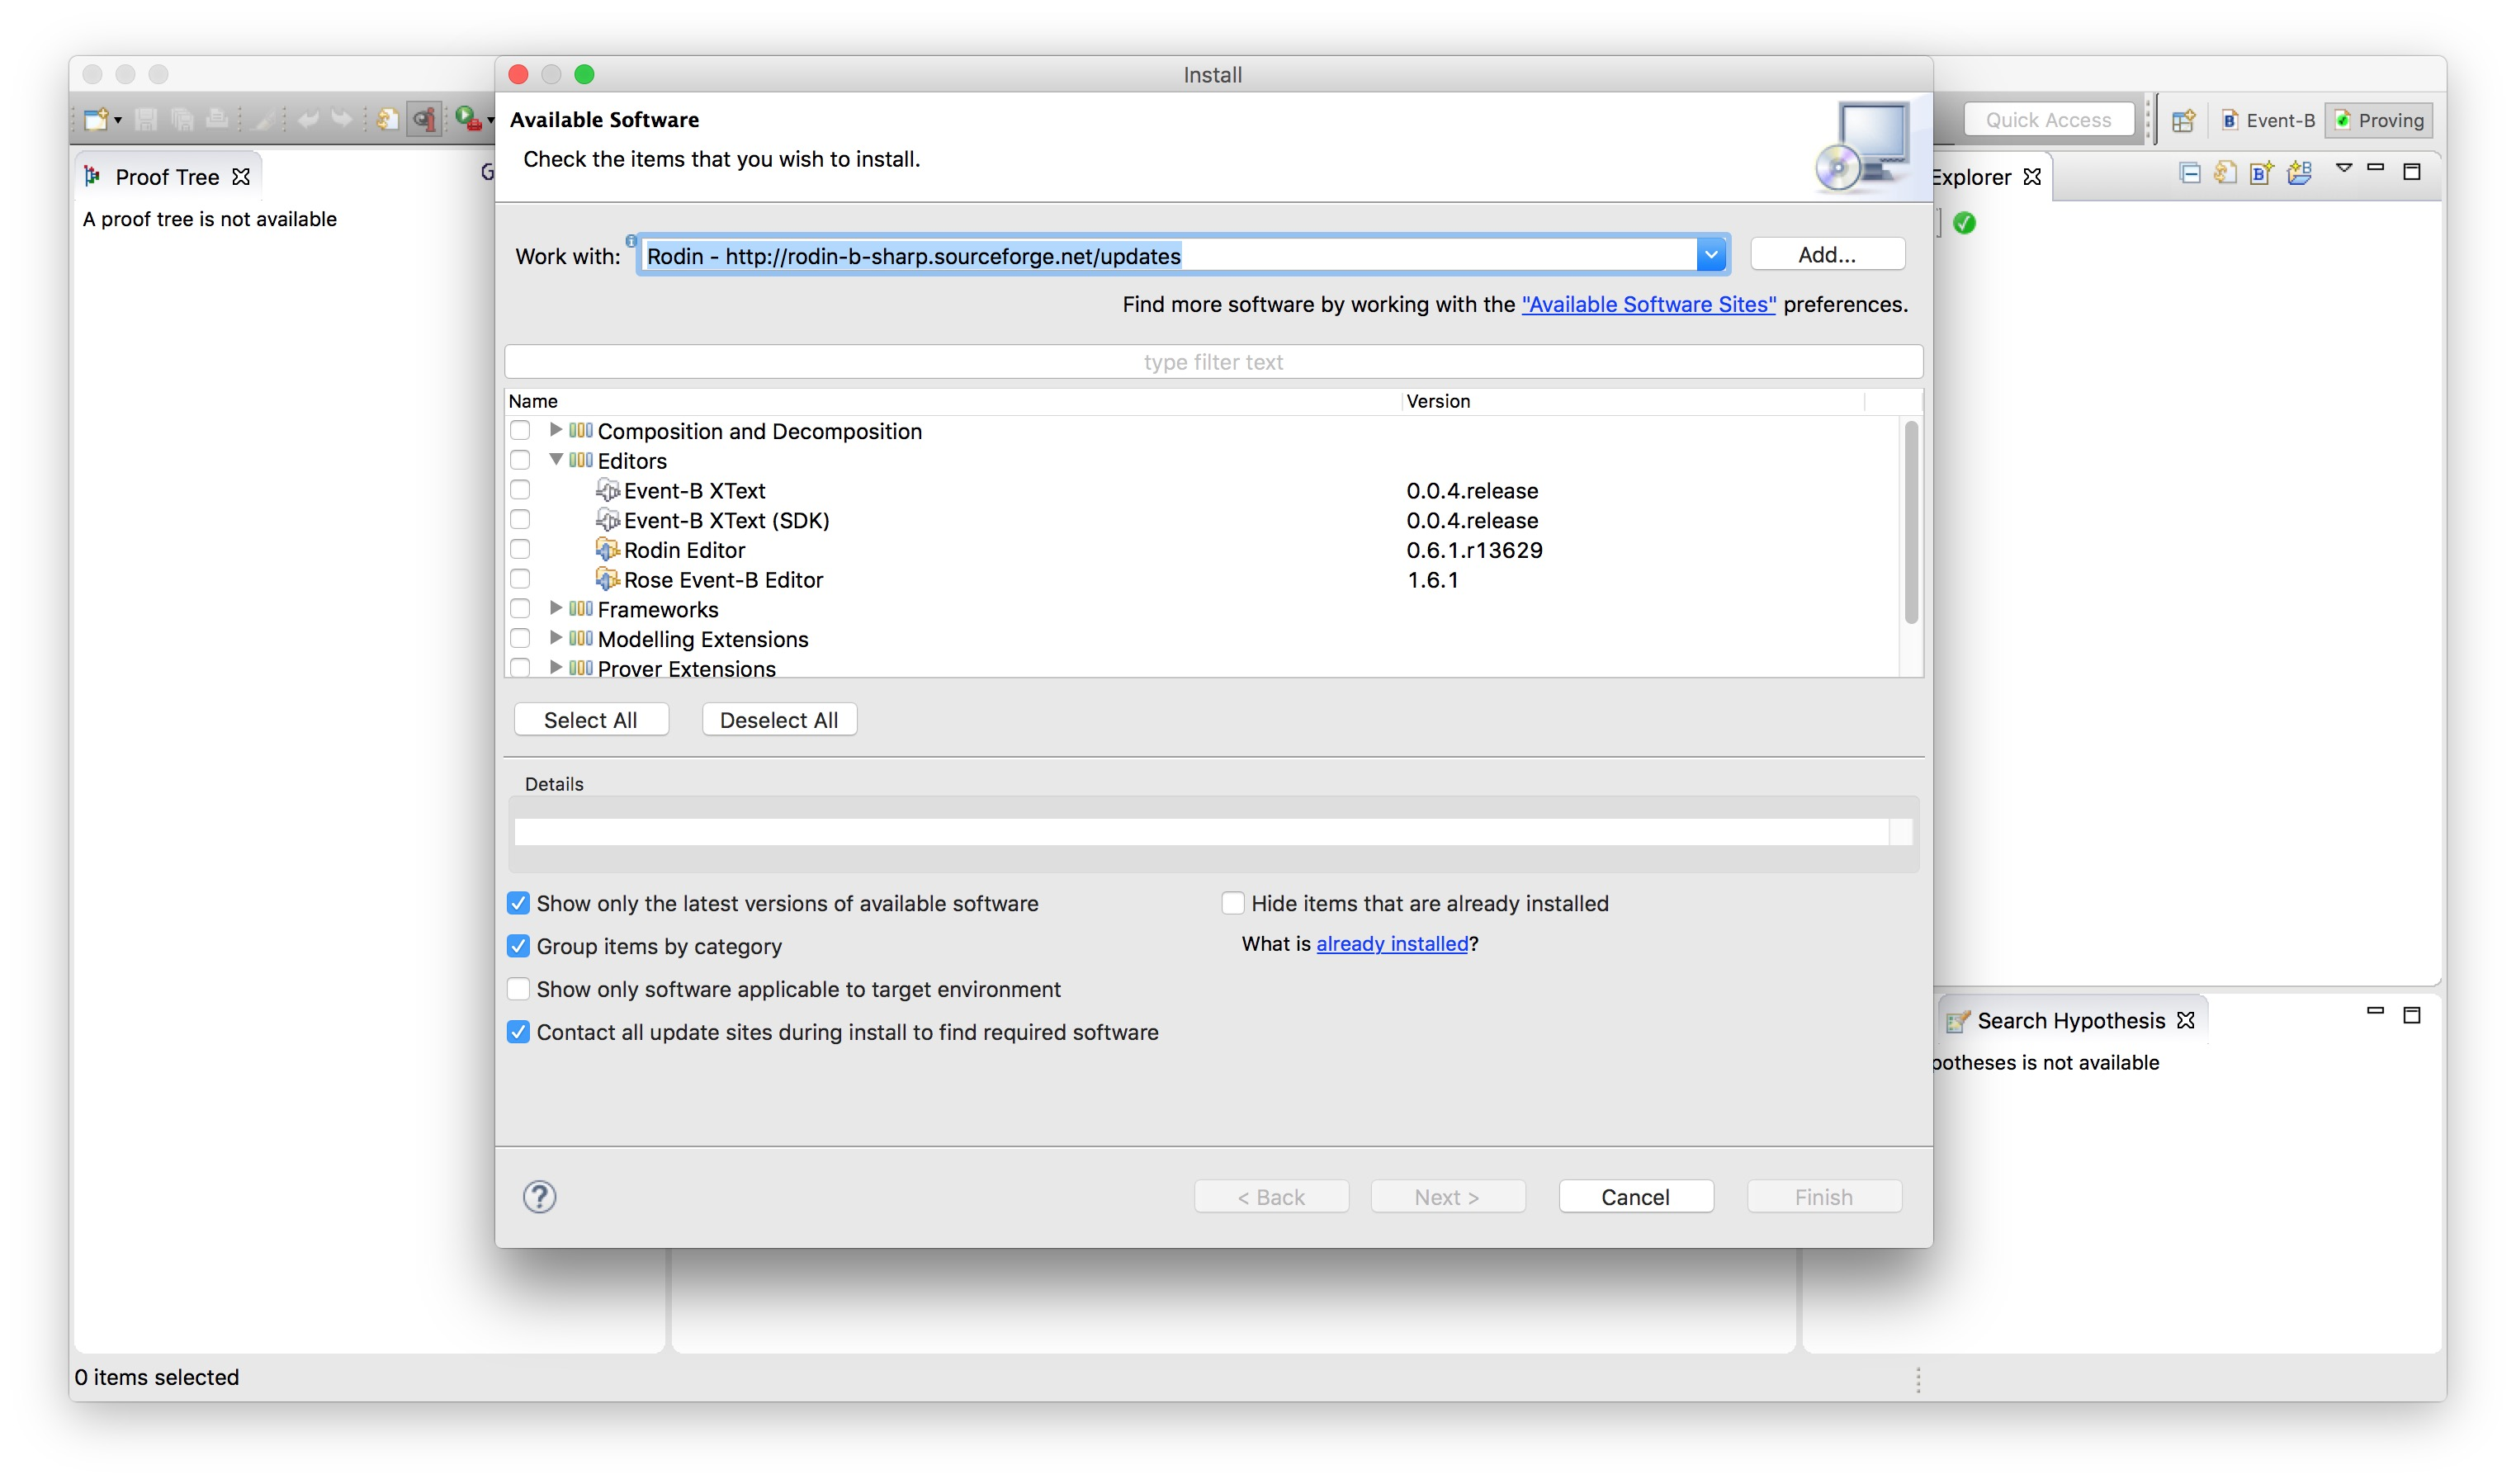
\includegraphics[width=512]{figures/EventBXTextInstallation}
  \else
  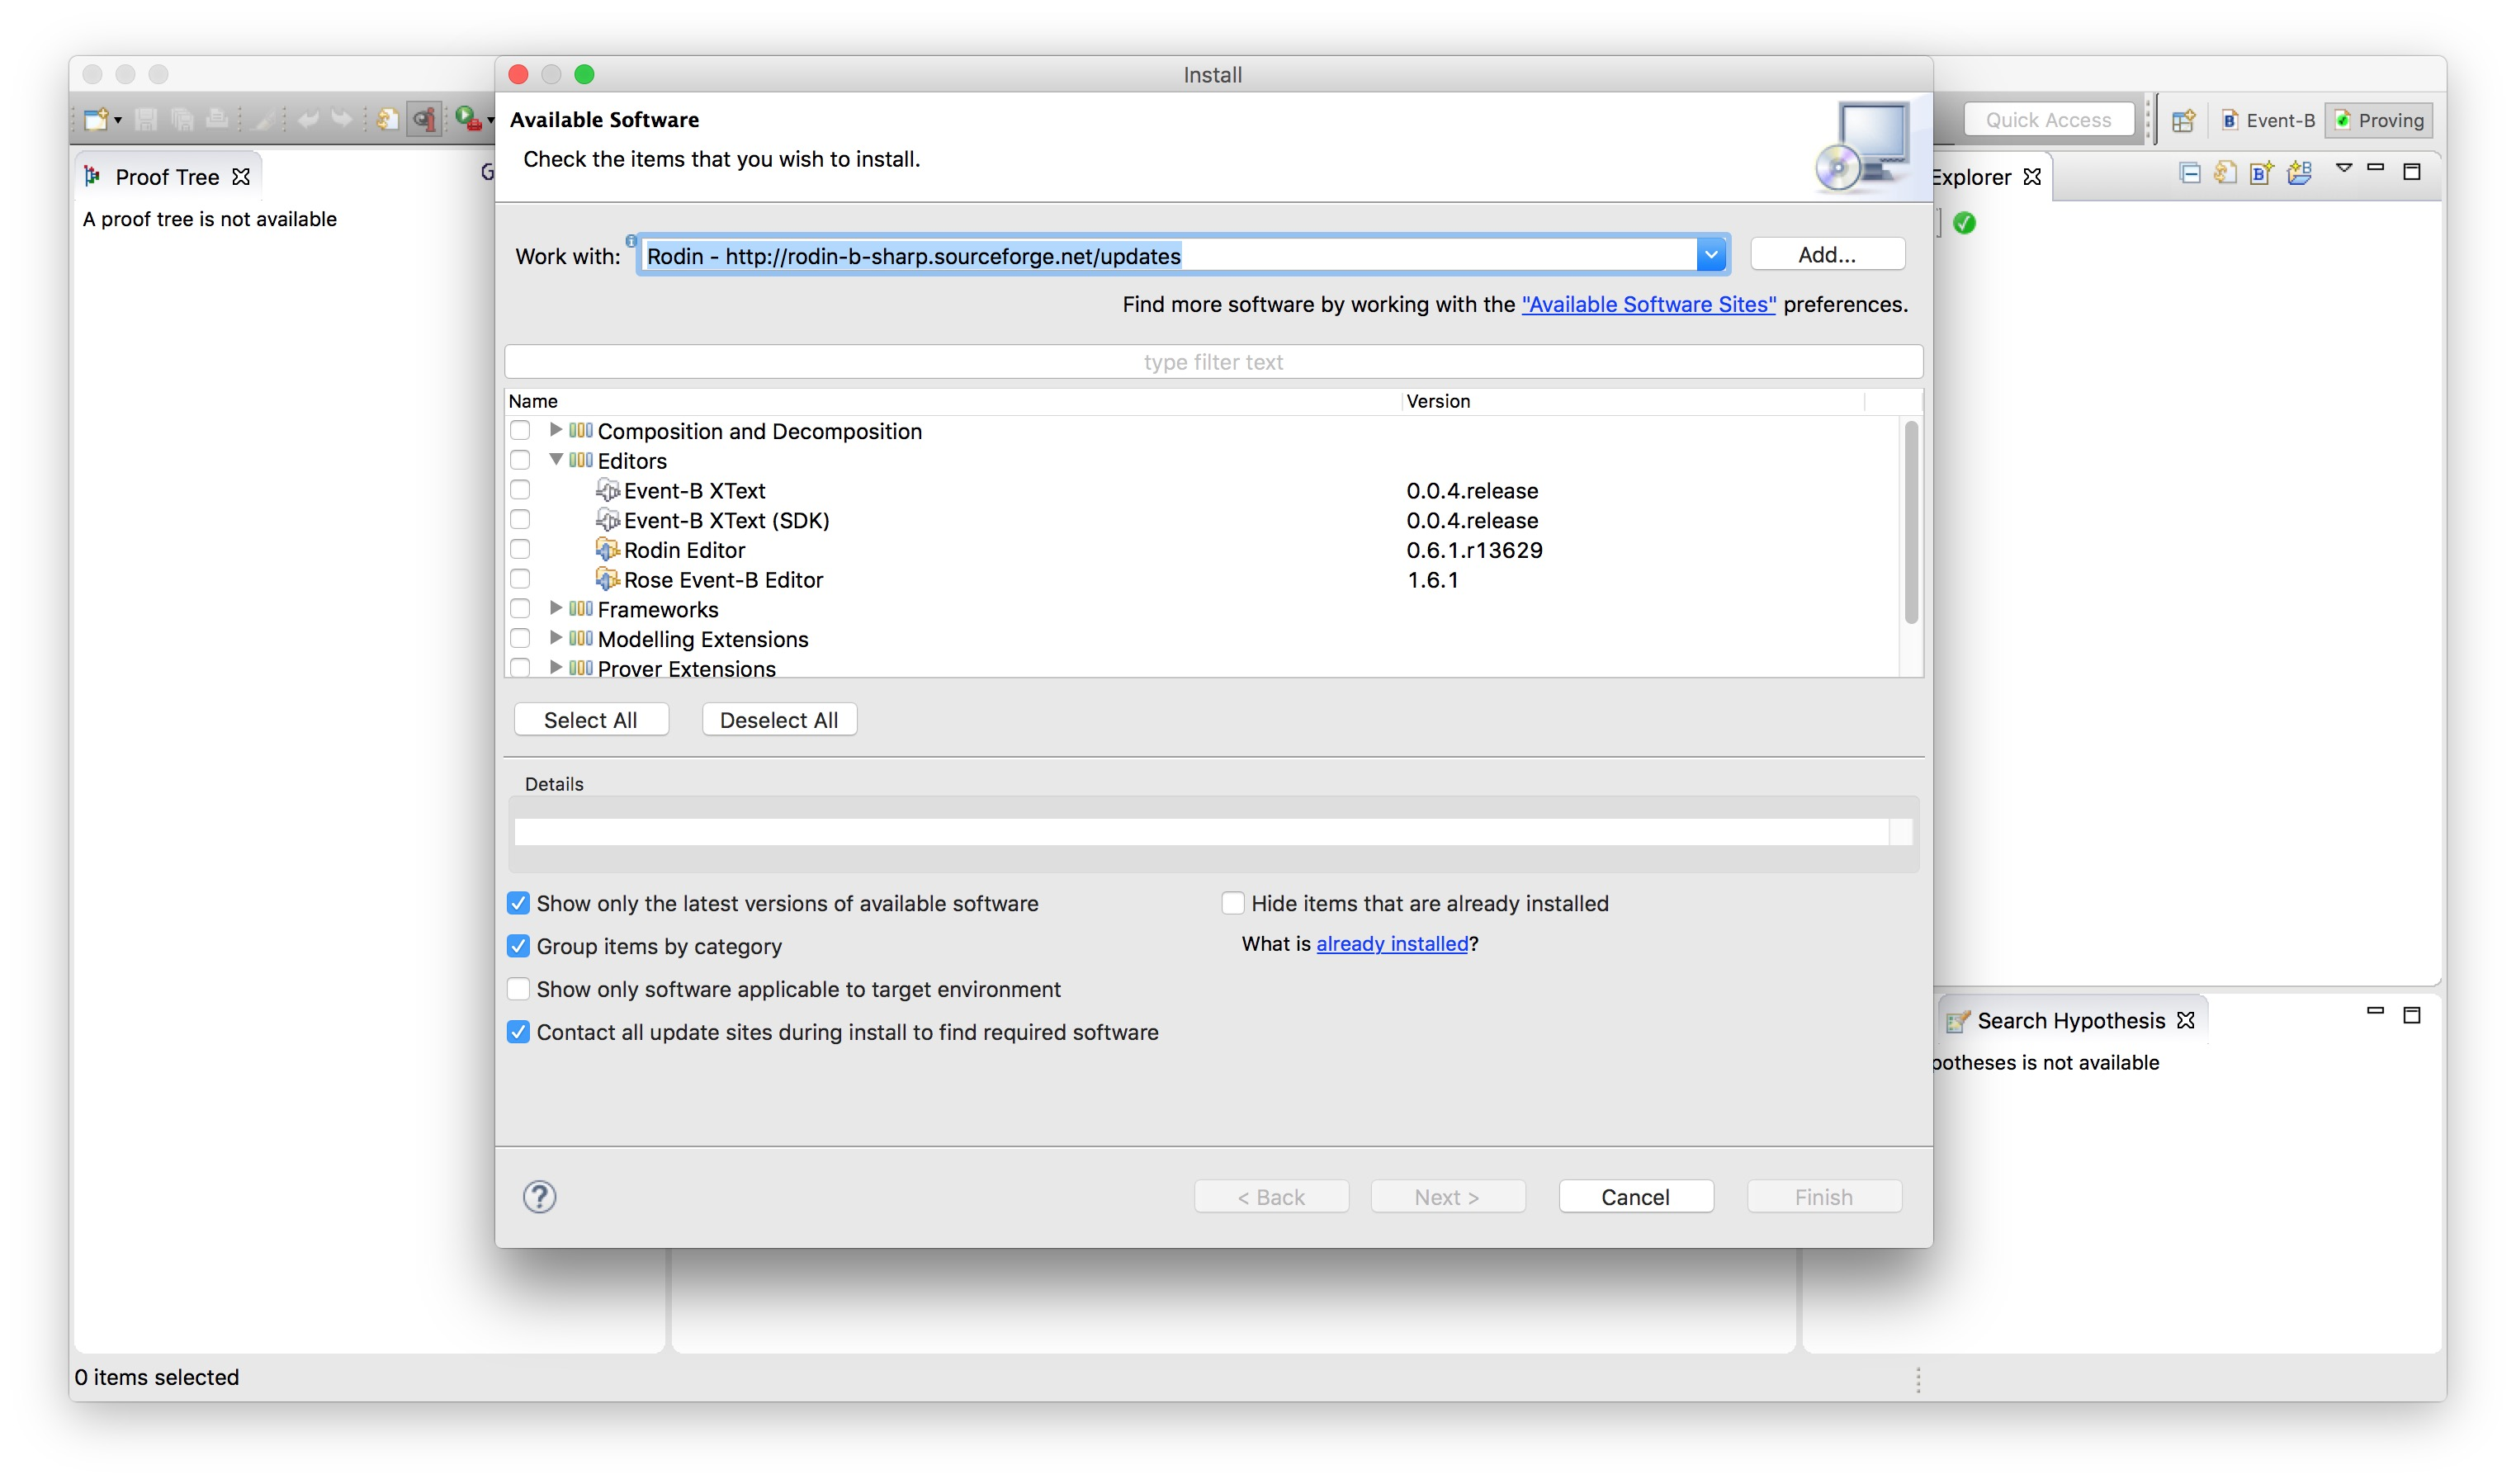
\includegraphics[width=0.9\textwidth]{figures/EventBXTextInstallation}
  \fi
  \caption{Adding XText Update Site}
  \label{fig:EventBXText-installation}
\end{figure}

\end{itemize}

\subsubsection{Release Notes}
\label{sec:release-notes}

\paragraph{0.0.5}
\begin{itemize}
\item Event-B XText Documentations (0.0.1): Documentation plug-in (Initial version).
\end{itemize}

\paragraph{0.0.4}
\begin{itemize}
\item Updated plug-in dependency for the feature
\end{itemize}

\paragraph{0.0.3}
\begin{itemize}
\item Event-B XText Context (0.0.3):
  \begin{itemize}
  \item Issue \#3: Single-line comment after the element, multi-line comment before
    the element
  \end{itemize}

\item Event-B XText Context IDE (0.0.2): Regenerated
 
\item Event-B XText ContextUI IDE (0.0.2): Regenerated

\item Event-B XText Machine (0.0.3):
  \begin{itemize}
  \item Issue \#3: Single-line comment after the element, multi-line comment before
    the element.

  \item Issue \#5: Event terminator using 'end' keyword instead of ';'
  \end{itemize}

\item Event-B XText Machine IDE (0.0.2) Regenerated
  
\item Event-B XText Machine UI IDE (0.0.2) Regenerated
\end{itemize}


\paragraph{0.0.2}
\begin{itemize}
\item Event-B XText Common (0.0.2):
  \begin{itemize}
  \item Added transient value service for XContext and XMachine.
  \end{itemize}

\item Event-B XText Context (0.0.2):
  \begin{itemize}
  \item Added formatter (used for auto-indentation).
  \end{itemize}

\item Event-B XText Machine (0.0.2):
  \begin{itemize}
  \item Added formatter (used for auto-indentation).
  \end{itemize}

\item Event-B XText UI (0.0.1): Initial version
  \begin{itemize}
  \item Added context menu for converting machines and contexts to XText.
  \end{itemize}
\end{itemize}

\paragraph{0.0.1} Initial version contains the following plug-ins:
\begin{itemize}
\item Event-B XText Branding (0.0.1) Initial version: Branding information

\item Event-B XText Common (0.0.1) Initial version: Common facilities

\item Event-B XText Context (0.0.1) Initial version: Core support for Event-B contexts

\item Event-B XText Context IDE (0.0.1) Initial version: IDE for Event-B contexts

\item Event-B XText Context UI (0.0.1) Initial version: UI for Event-B contexts

\item Event-B XText Machine (0.0.1) Initial version: Core support for Event-B machines

\item Event-B XText Machine IDE (0.0.1) Initial version: IDE for Event-B machines

\item Event-B XText Machine UI (0.0.1) Initial version: UI for Event-B machines
\end{itemize}

\subsubsection{IMPORTANT}
\label{sec:important}

\begin{itemize}
\item Currently, Event-B XText front-end ONLY supports ``standard'' Event-B machines and contexts.

\item Since the XContexts and XMachines are compiled to the Rodin files, the corresponding Rodin contexts and machines will be \textbf{OVER-WRITTEN}. Any changes in the Rodin files will not be lost.

\item \textbf{DO NOT USE} the Event-B XText Front-end if you use modelling plug-ins such as \emph{iUML-B} state-machines and class-diagrams, as the additional modelling elements will be over-written.
\end{itemize}

\subsubsection{Known Issues}
\label{sec:known-issues}

\begin{itemize}
\item Converting to XText: Currently, the ``extended'' attribute of events are not serialised.
\end{itemize}

\subsubsection{Configuration}
\label{sec:configuration}

\paragraph{Event-B Explorer}
By default, XContext files (extension .bucx) and XMachine files (extension .bumx) are not display in the \emph{Event-B Explorer}. To enable this, select \emph{Customize view} for \emph{Event-B Explorer} and uncheck the option \emph{All files and folders}.

\subsection{Basic Tutorial}
\label{sec:basic-tutorial}

This tutorial provides a step-by-step walk-through working with XEvent-B constructs. This tutorial also available as Cheatsheets with the Rodin Platform (\texttt{Help/Cheat Sheets/Event-B XText Cheatsheets/Event-B XText Basic Tutorial}).

\subsubsection{Task 1. Customise the Event-B Explorer}
\textbf{Introduction}
The purpose of this task is to customise the Event-B Explorer so that XEvent-B constructs are visible.
\begin{description}
\item[Step 1. Disable the filter on ``All files and folders''] Select ``Customize View'' of Event-B Explorer View. Make sure that ``All files and folders'' from the dialog is \textbf{Unchecked}.
\end{description}

\textbf{Conclusion} Since the filter on ``All files and folders'' is now disabled, there might be other files and folders than XEvent-B constructs will also be visible in the Event-B Explorer.

\subsubsection{Task 2. Create an Event-B Project}
\textbf{Introduction} The purpose of this task is to create an Event-B project for the XEvent-B constructs. 
\begin{description}
\item[Step 1. Create a new Event-B Project] Create a new Event-B Project named ``Club'' using the \emph{New Event-B Project} wizard (see Figure~\ref{fig:CreateProject}).
\begin{figure}[!htbp]
  \centering
  \ifplastex
  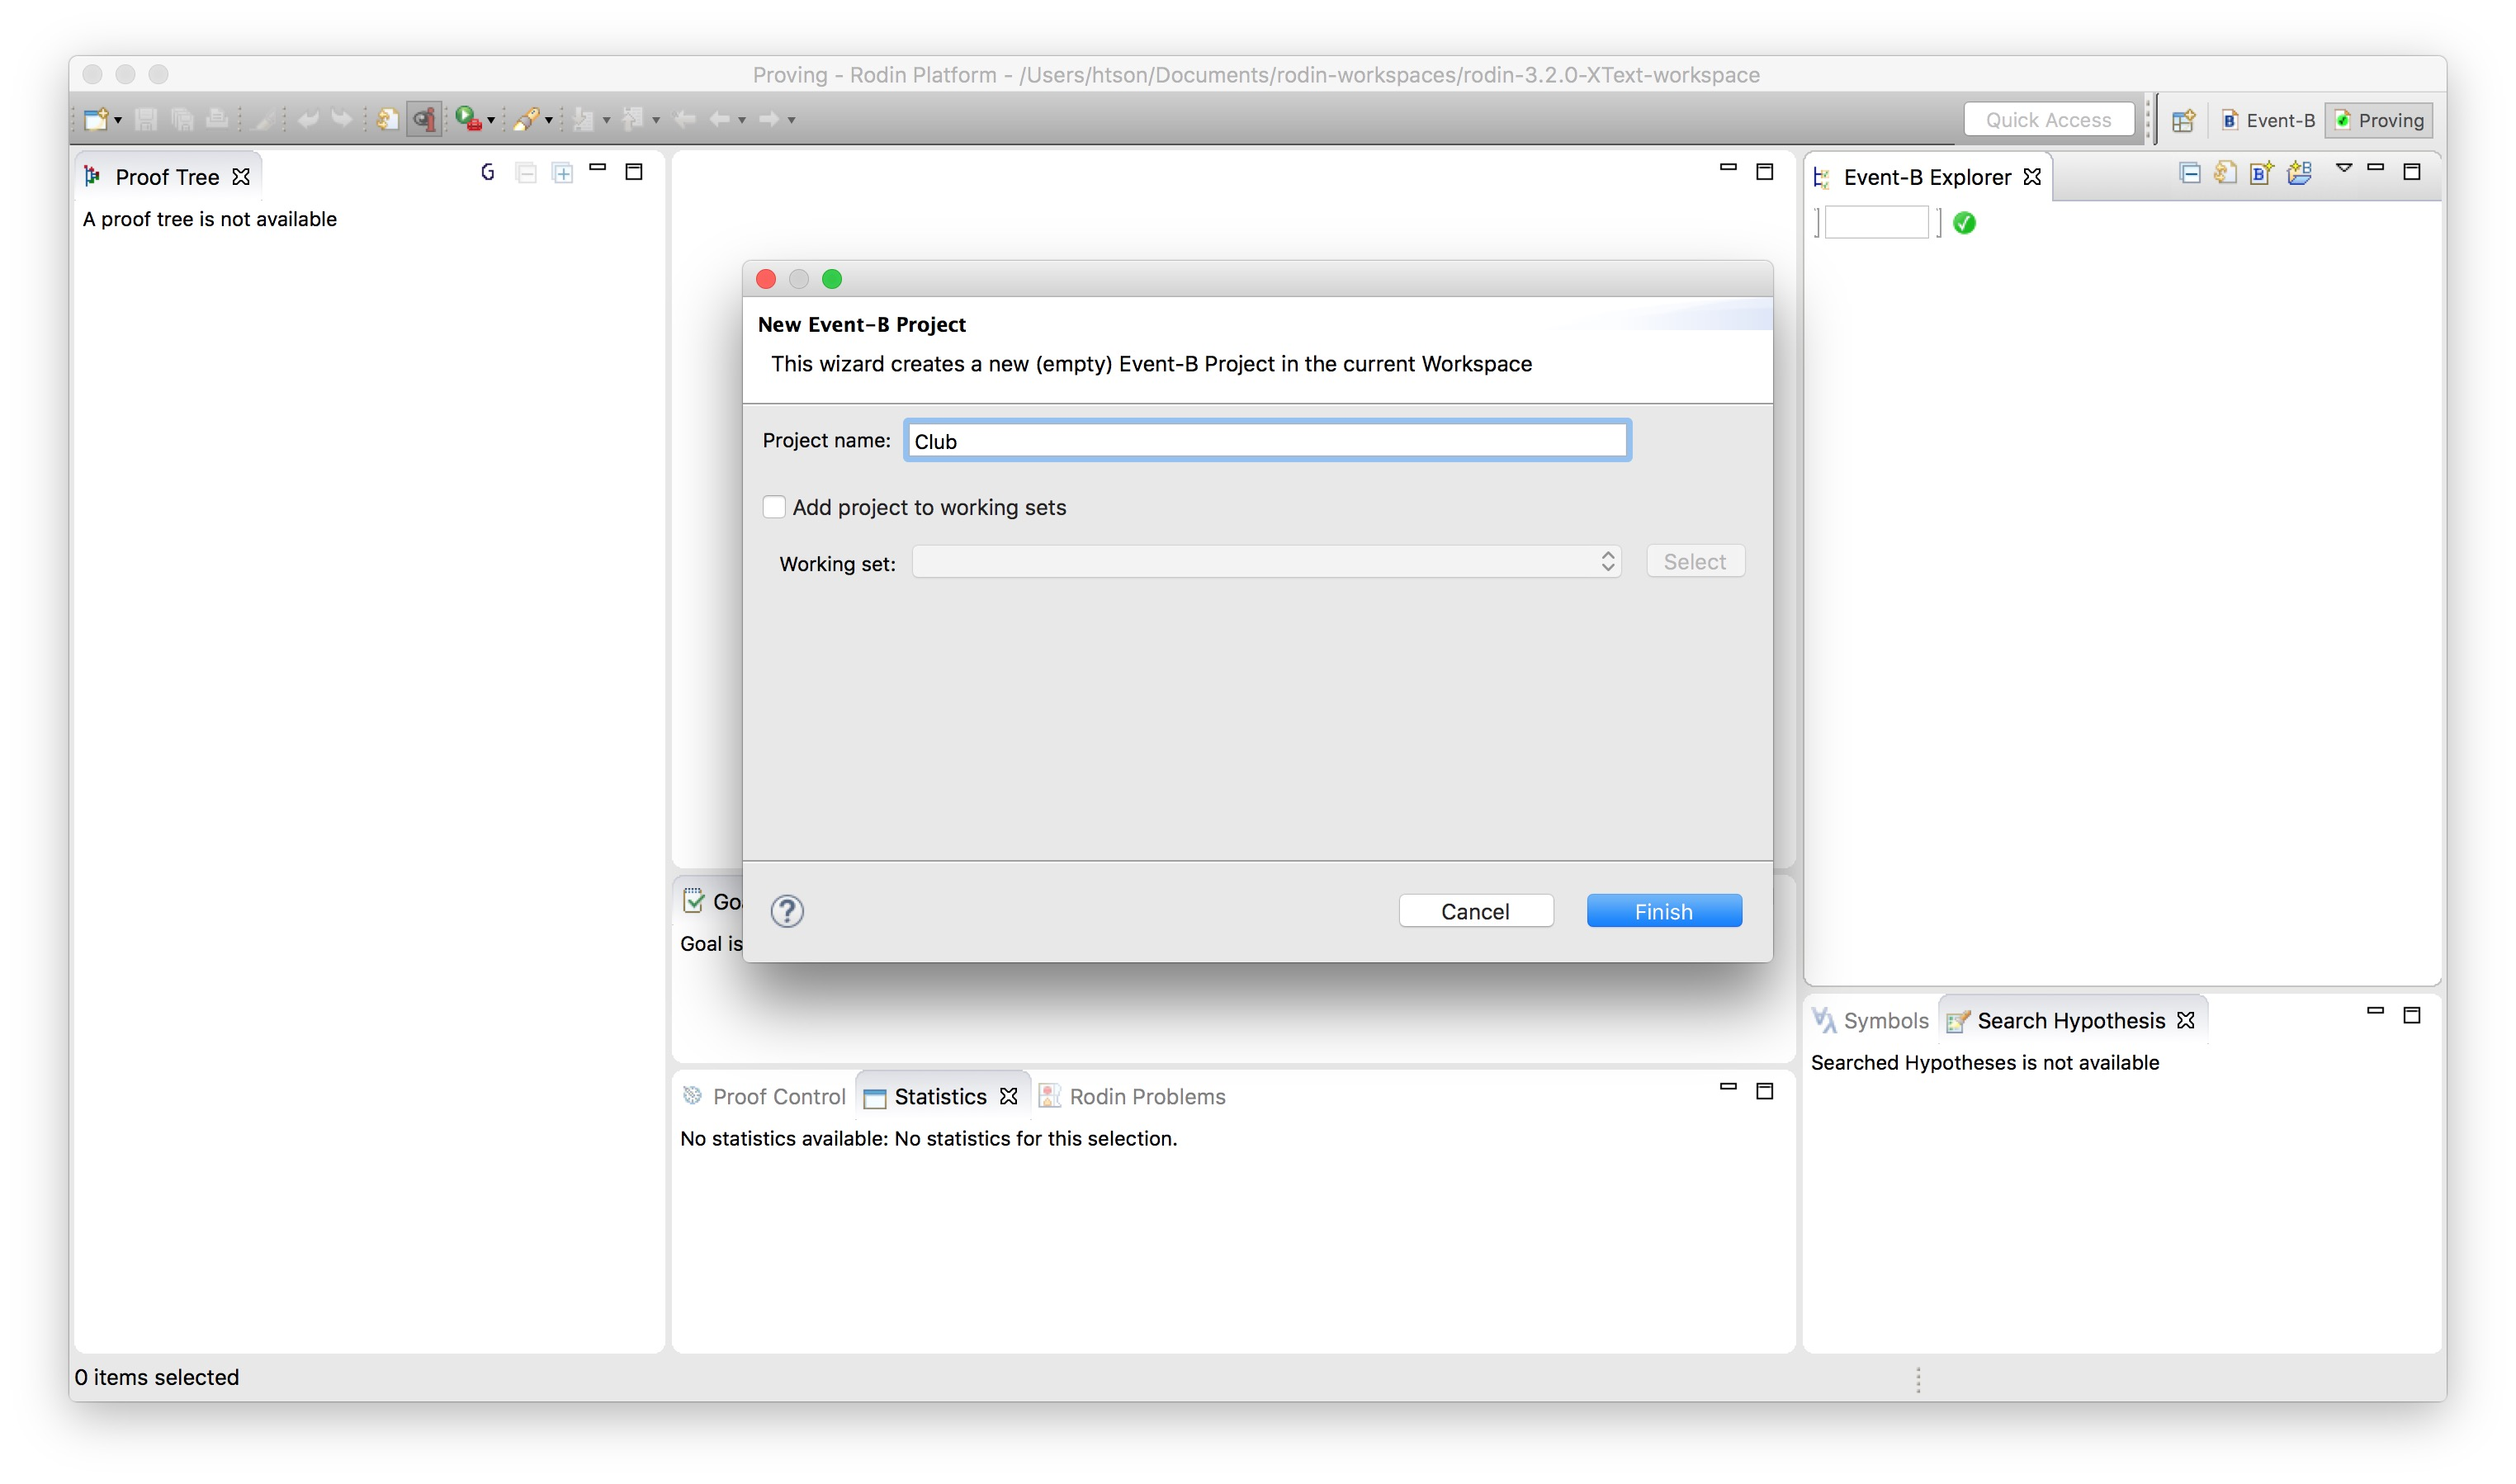
\includegraphics[width=512]{figures/CreateProject}
  \else
  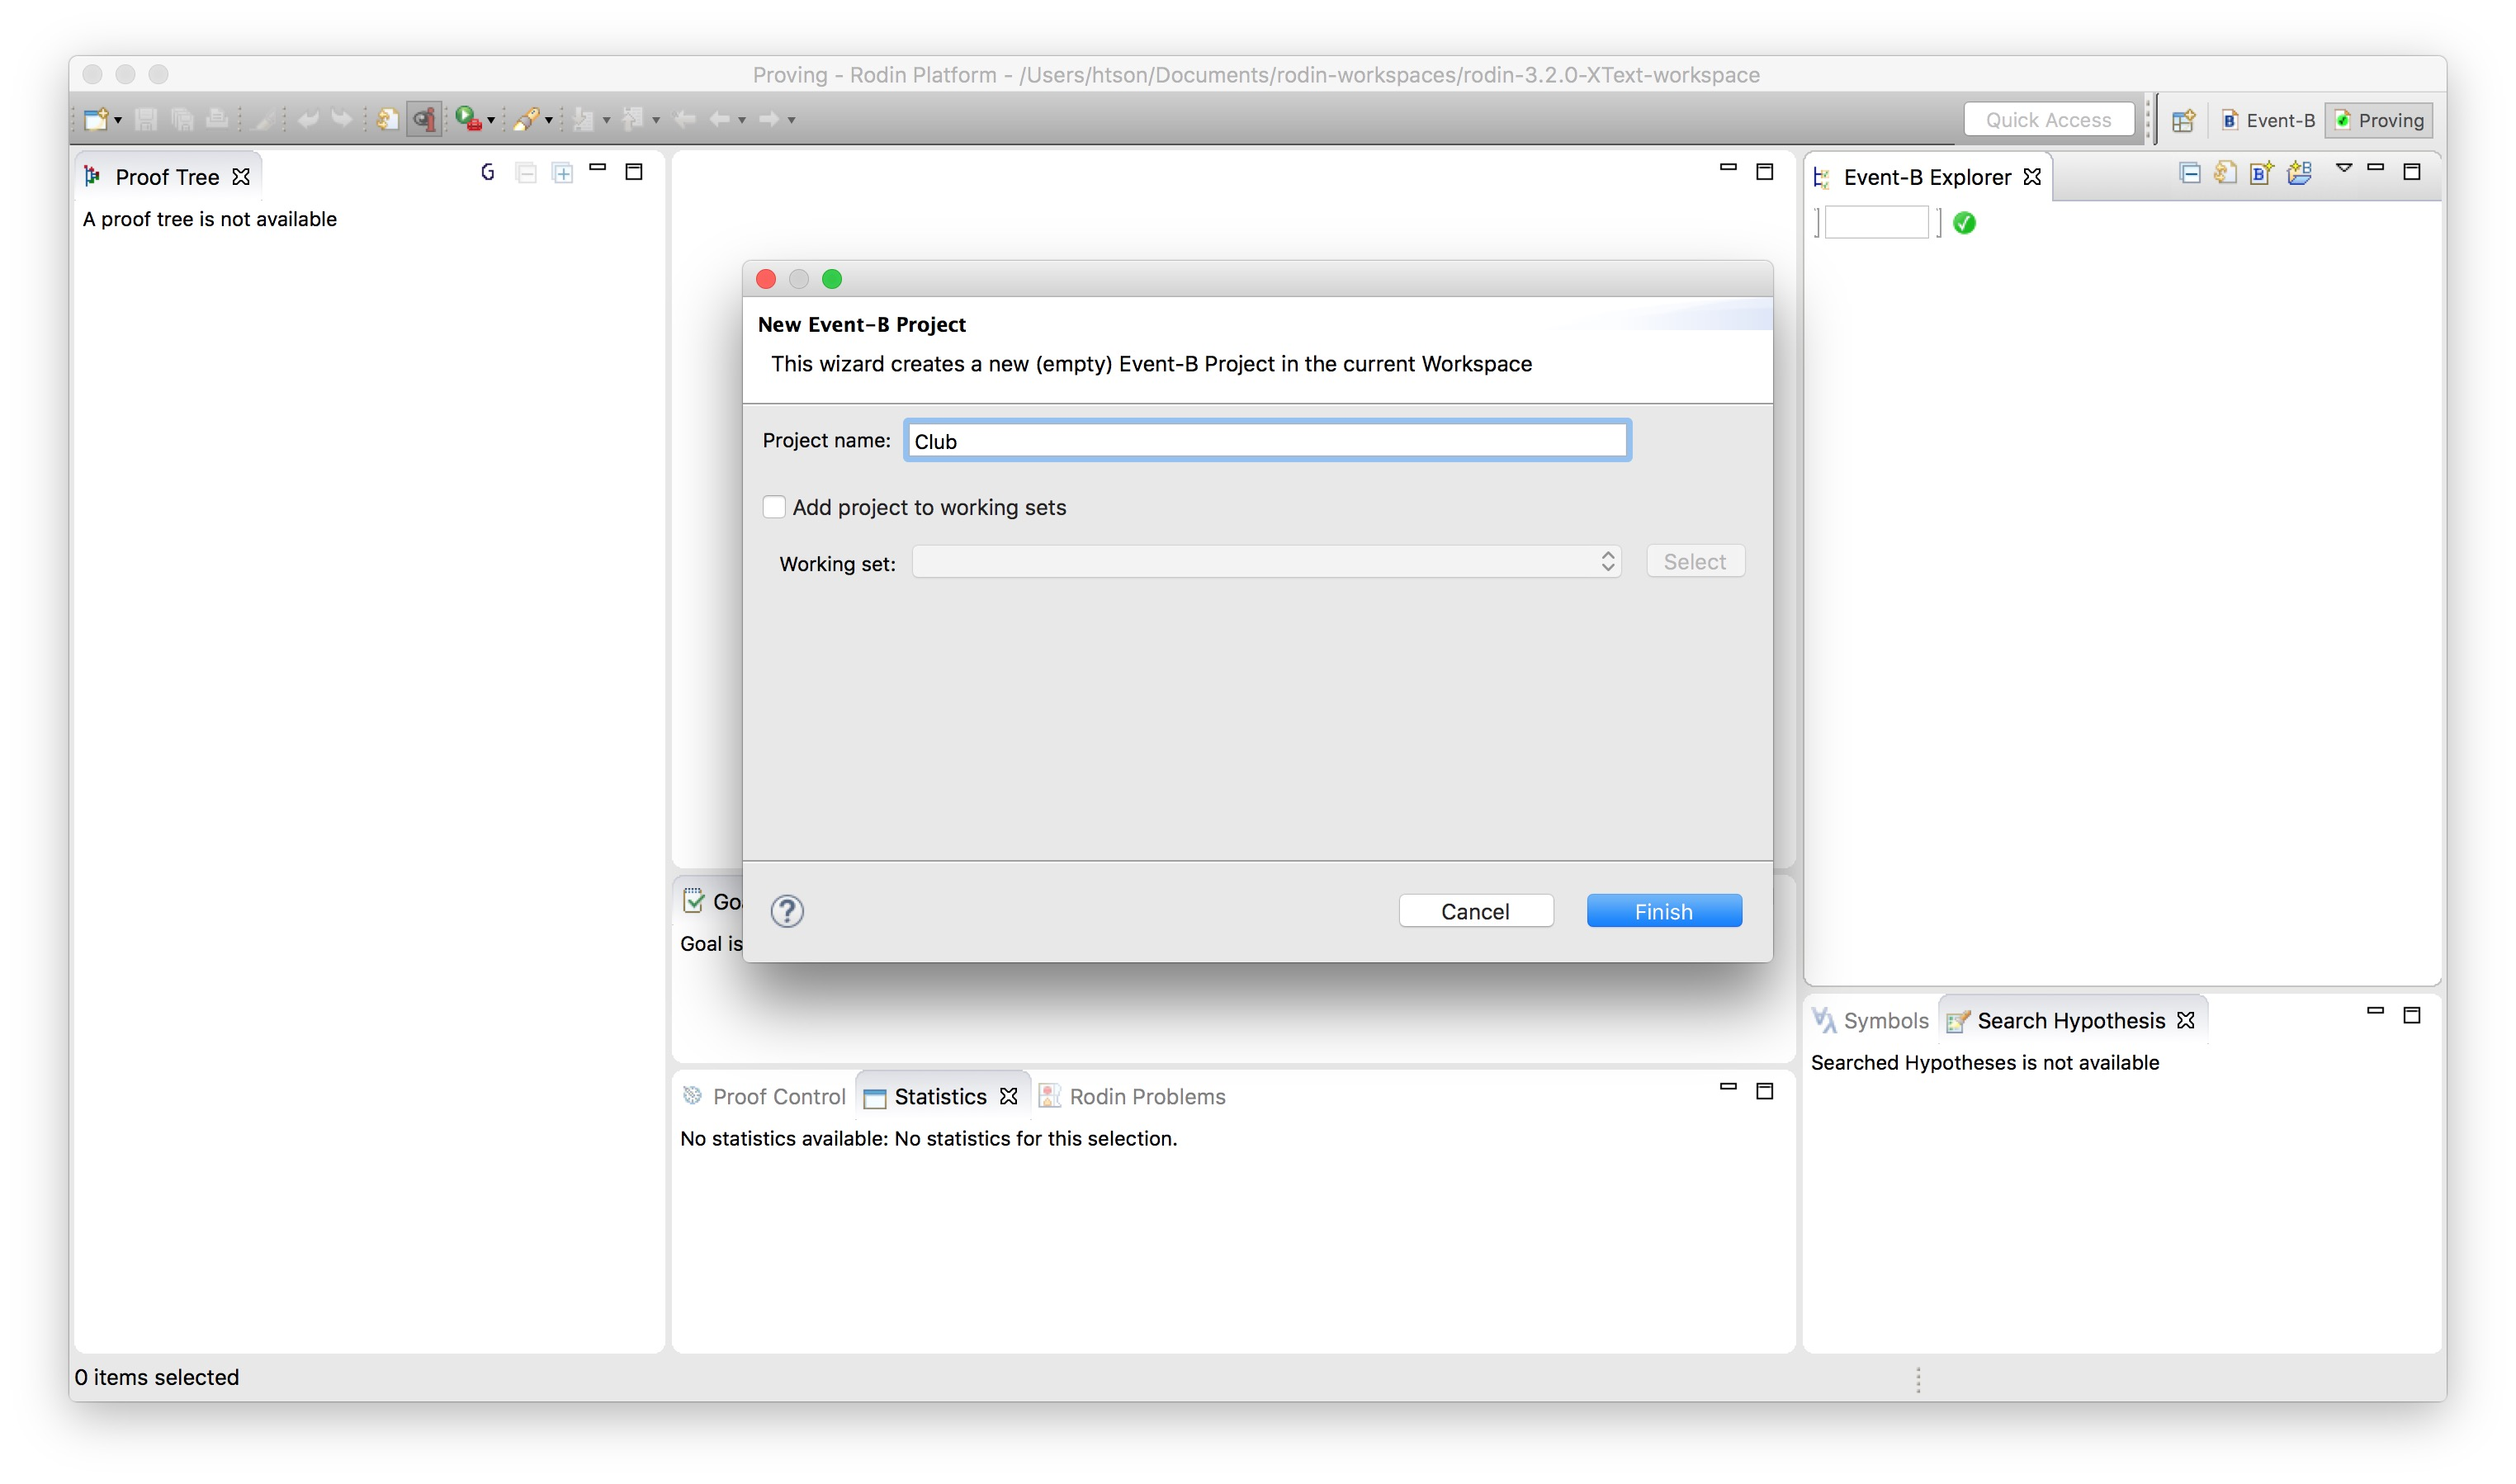
\includegraphics[width=0.9\textwidth]{figures/CreateProject}
  \fi
  \caption{Create Event-B Project called ``Club''}
  \label{fig:CreateProject}
\end{figure}

\end{description}
\textbf{Conclusion} By now, the project ``Club'' should be visible in the Event-B Explorer.


\subsubsection{Task 3. Create a simple XContext coursesCtx.bucx}
\textbf{Introduction} The purpose of this task is to create a simple XContext within the newly created project.
\begin{description}
\item[Step 1. Create a new XContext coursesCtx.bucx] Create a new XContext named ``coursesCtx.bucx'' using the \emph{New File wizard} (see Figure~\ref{fig:CreateCoursesCtx}).
         \textbf{Important}: A pop-up dialog will be displayed asking to convert the ``Club''
         project to XText project, please answer \textbf{Yes} (see Figure~\ref{fig:ConvertToXText}).
\begin{figure}[!htbp]
  \centering
  \ifplastex
  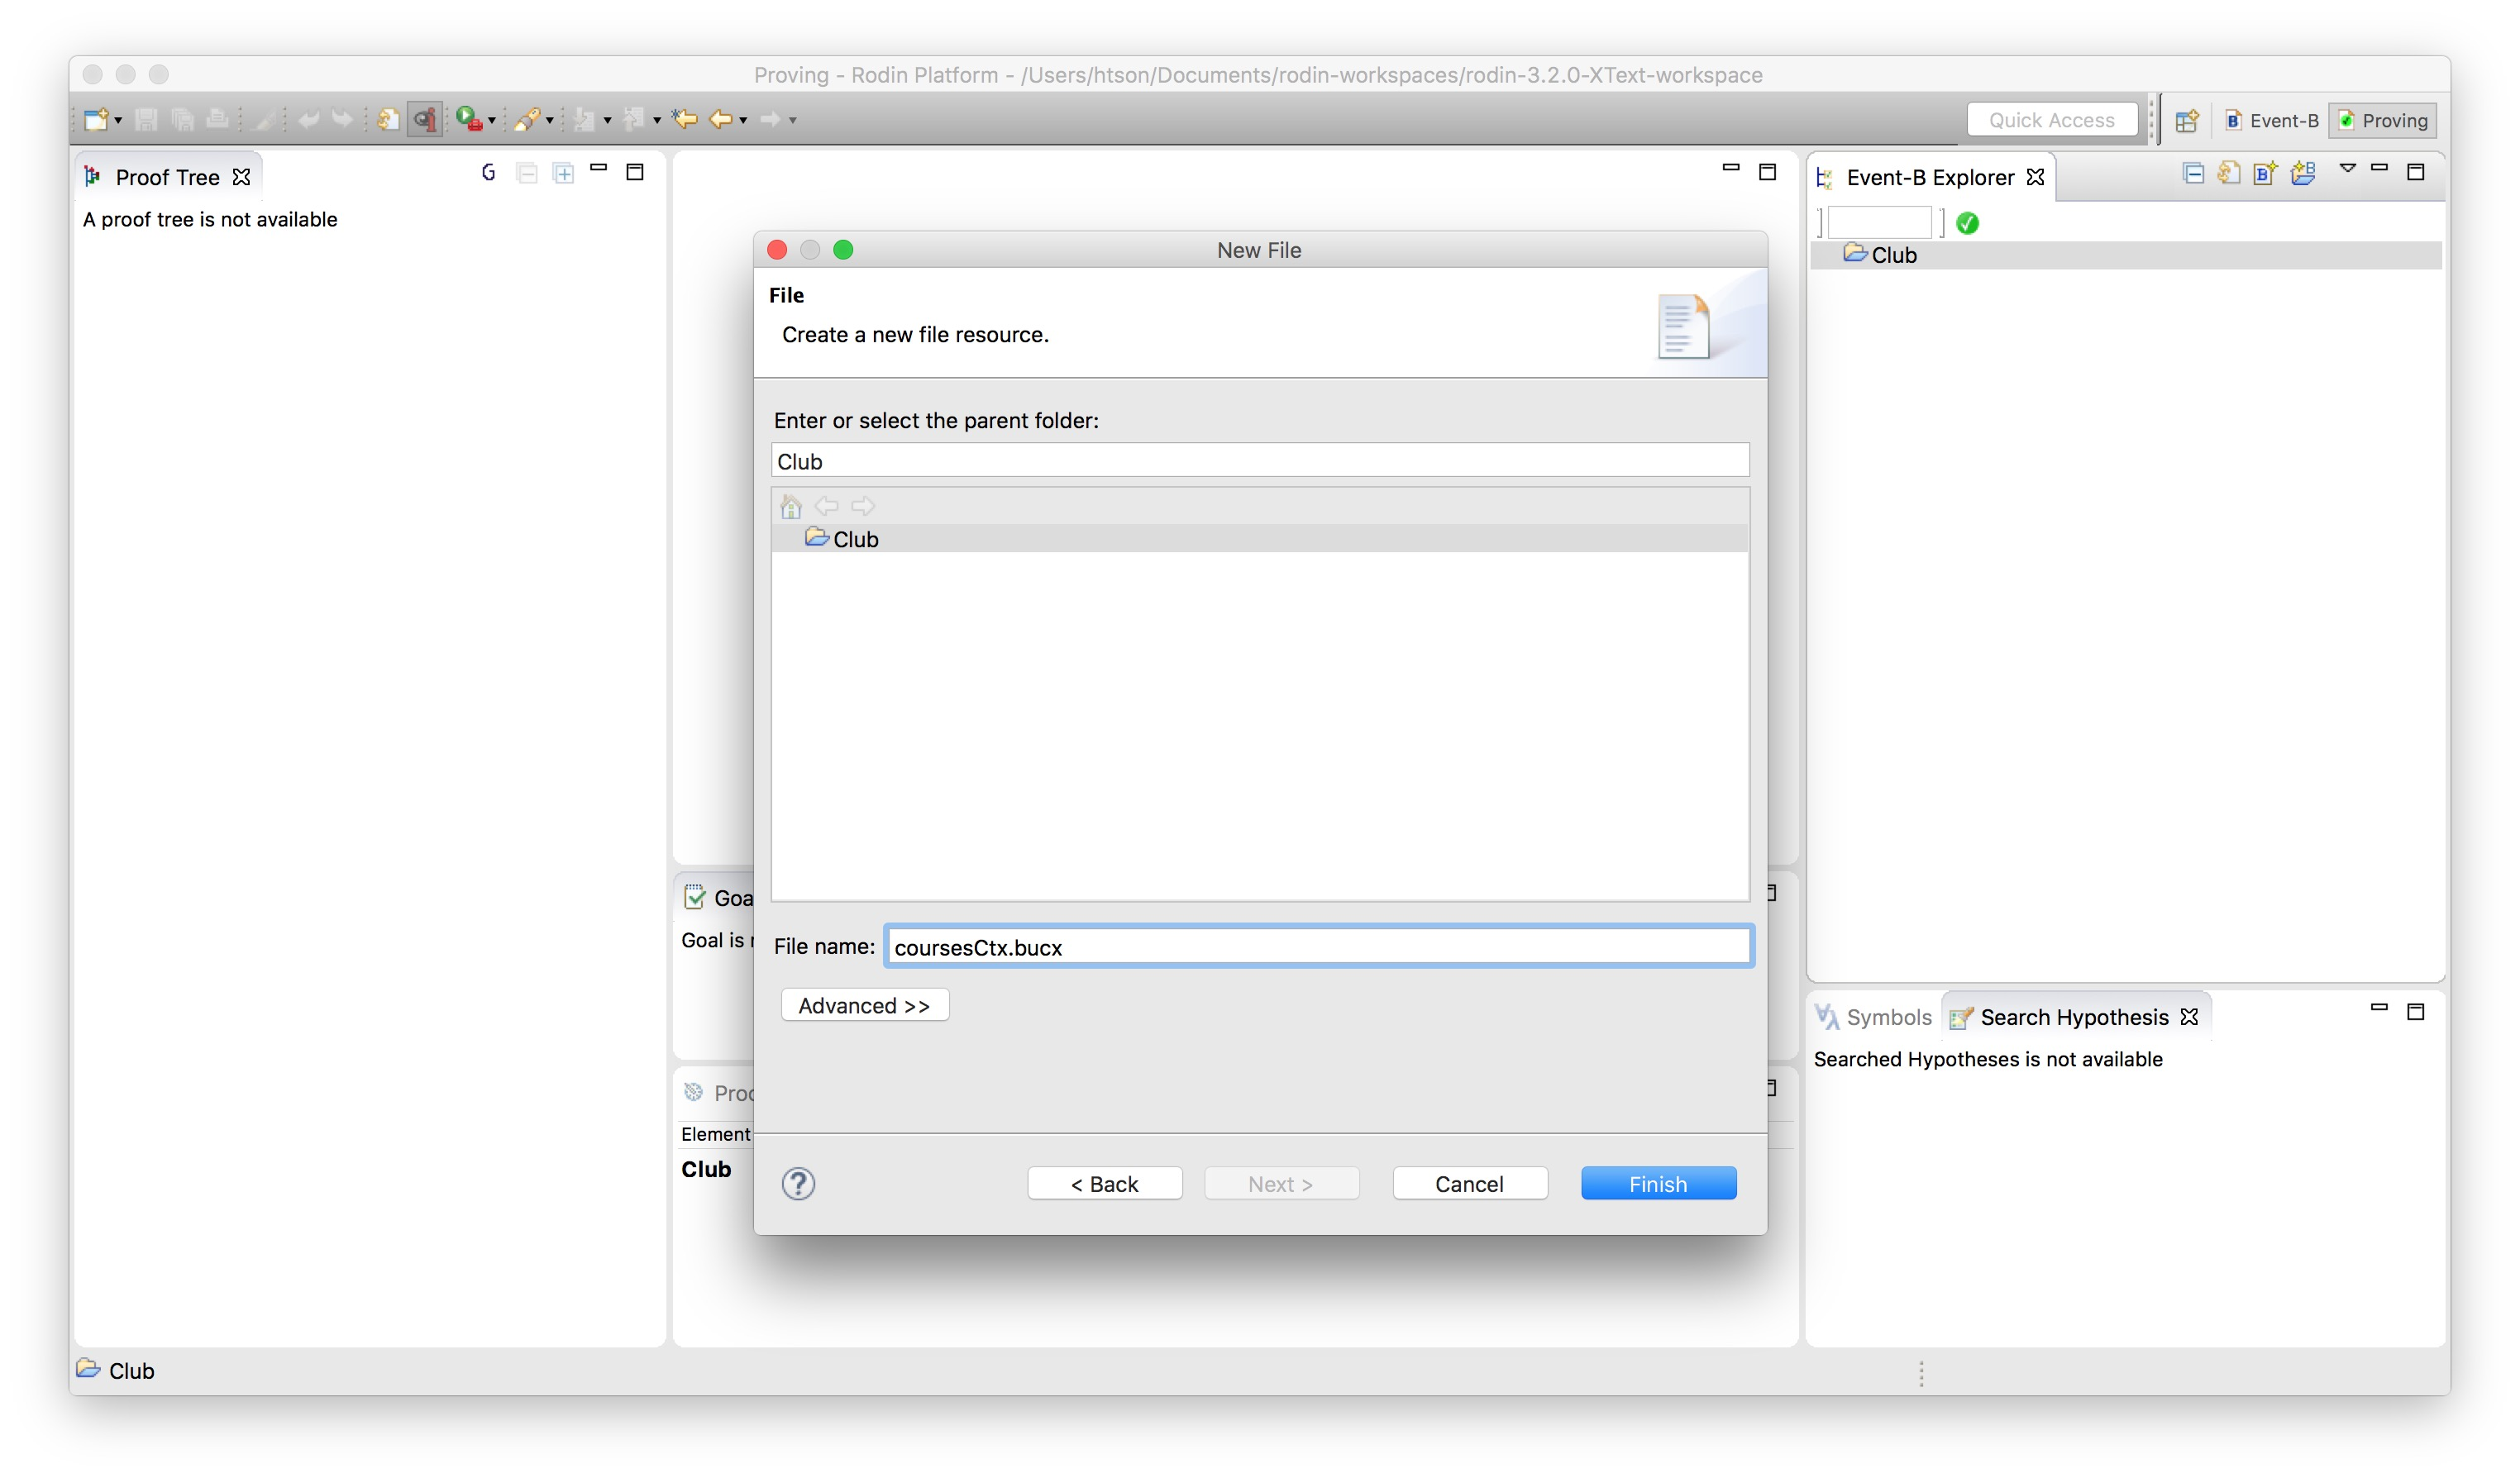
\includegraphics[width=512]{figures/CreateCoursesCtx}
  \else
  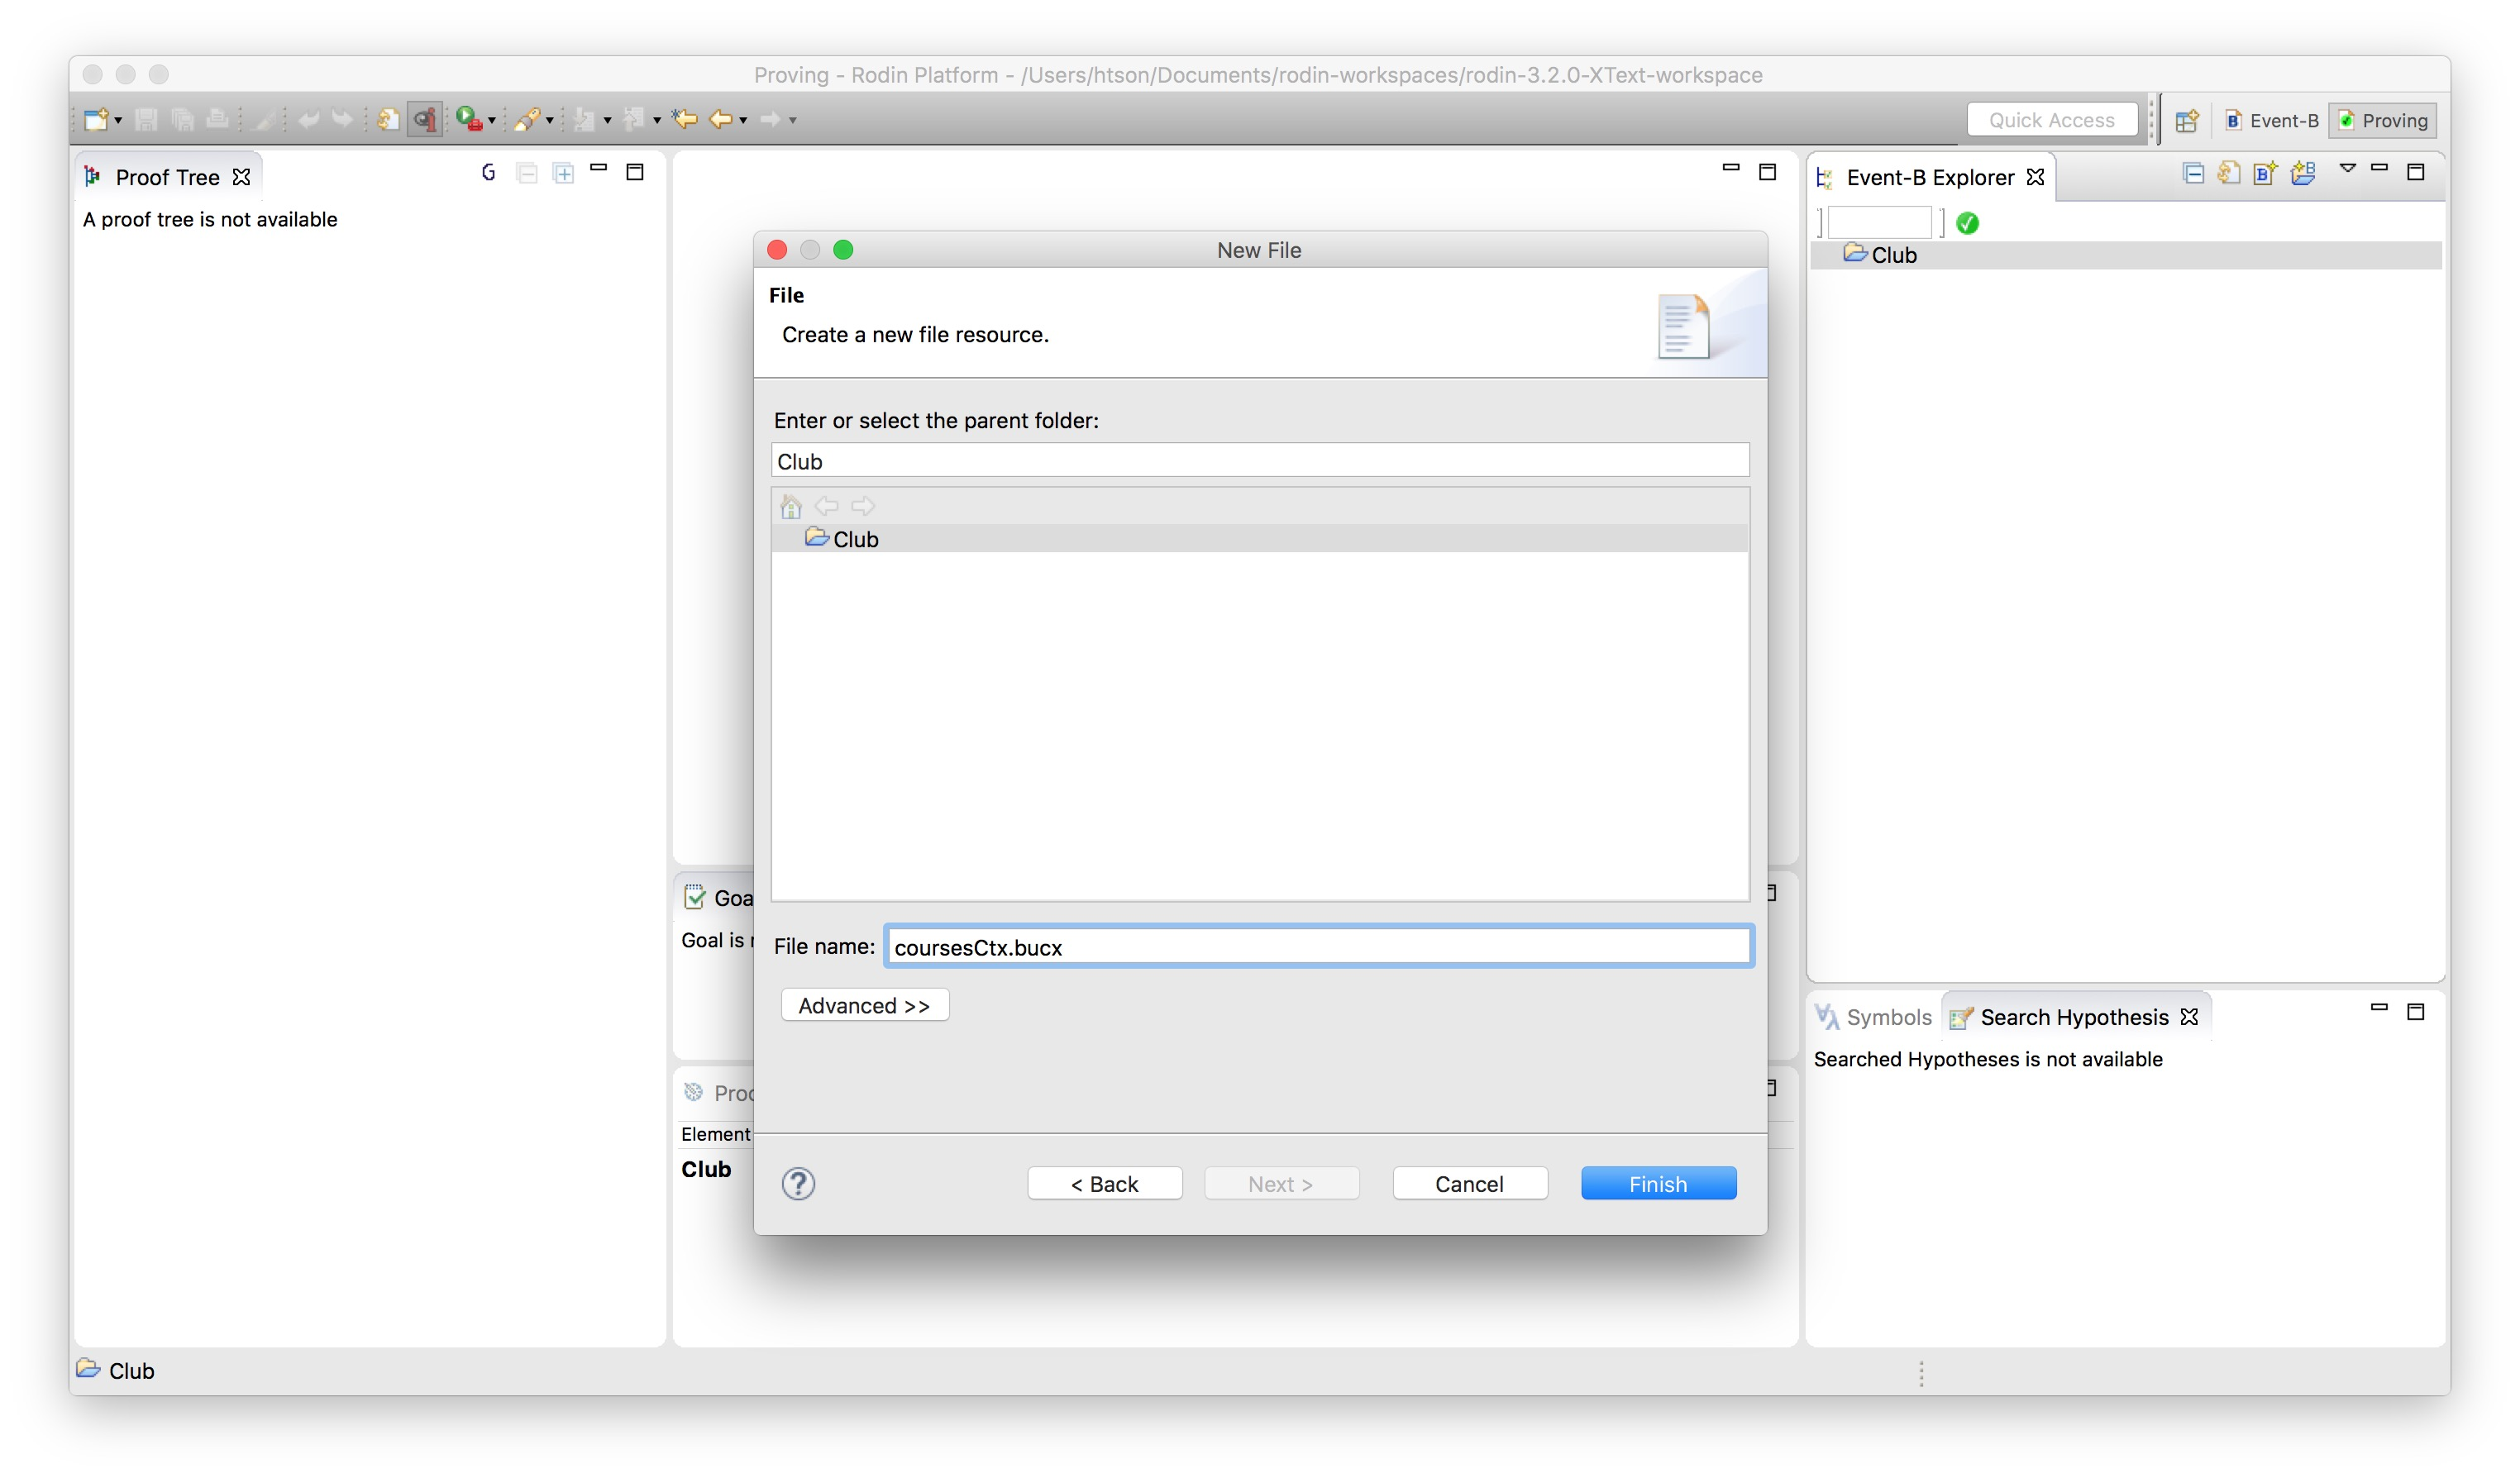
\includegraphics[width=0.9\textwidth]{figures/CreateCoursesCtx}
  \fi
  \caption{Create an XContext called ``coursesCtx.bucx''}
  \label{fig:CreateCoursesCtx}
\end{figure}
\begin{figure}[!htbp]
  \centering
  \ifplastex
  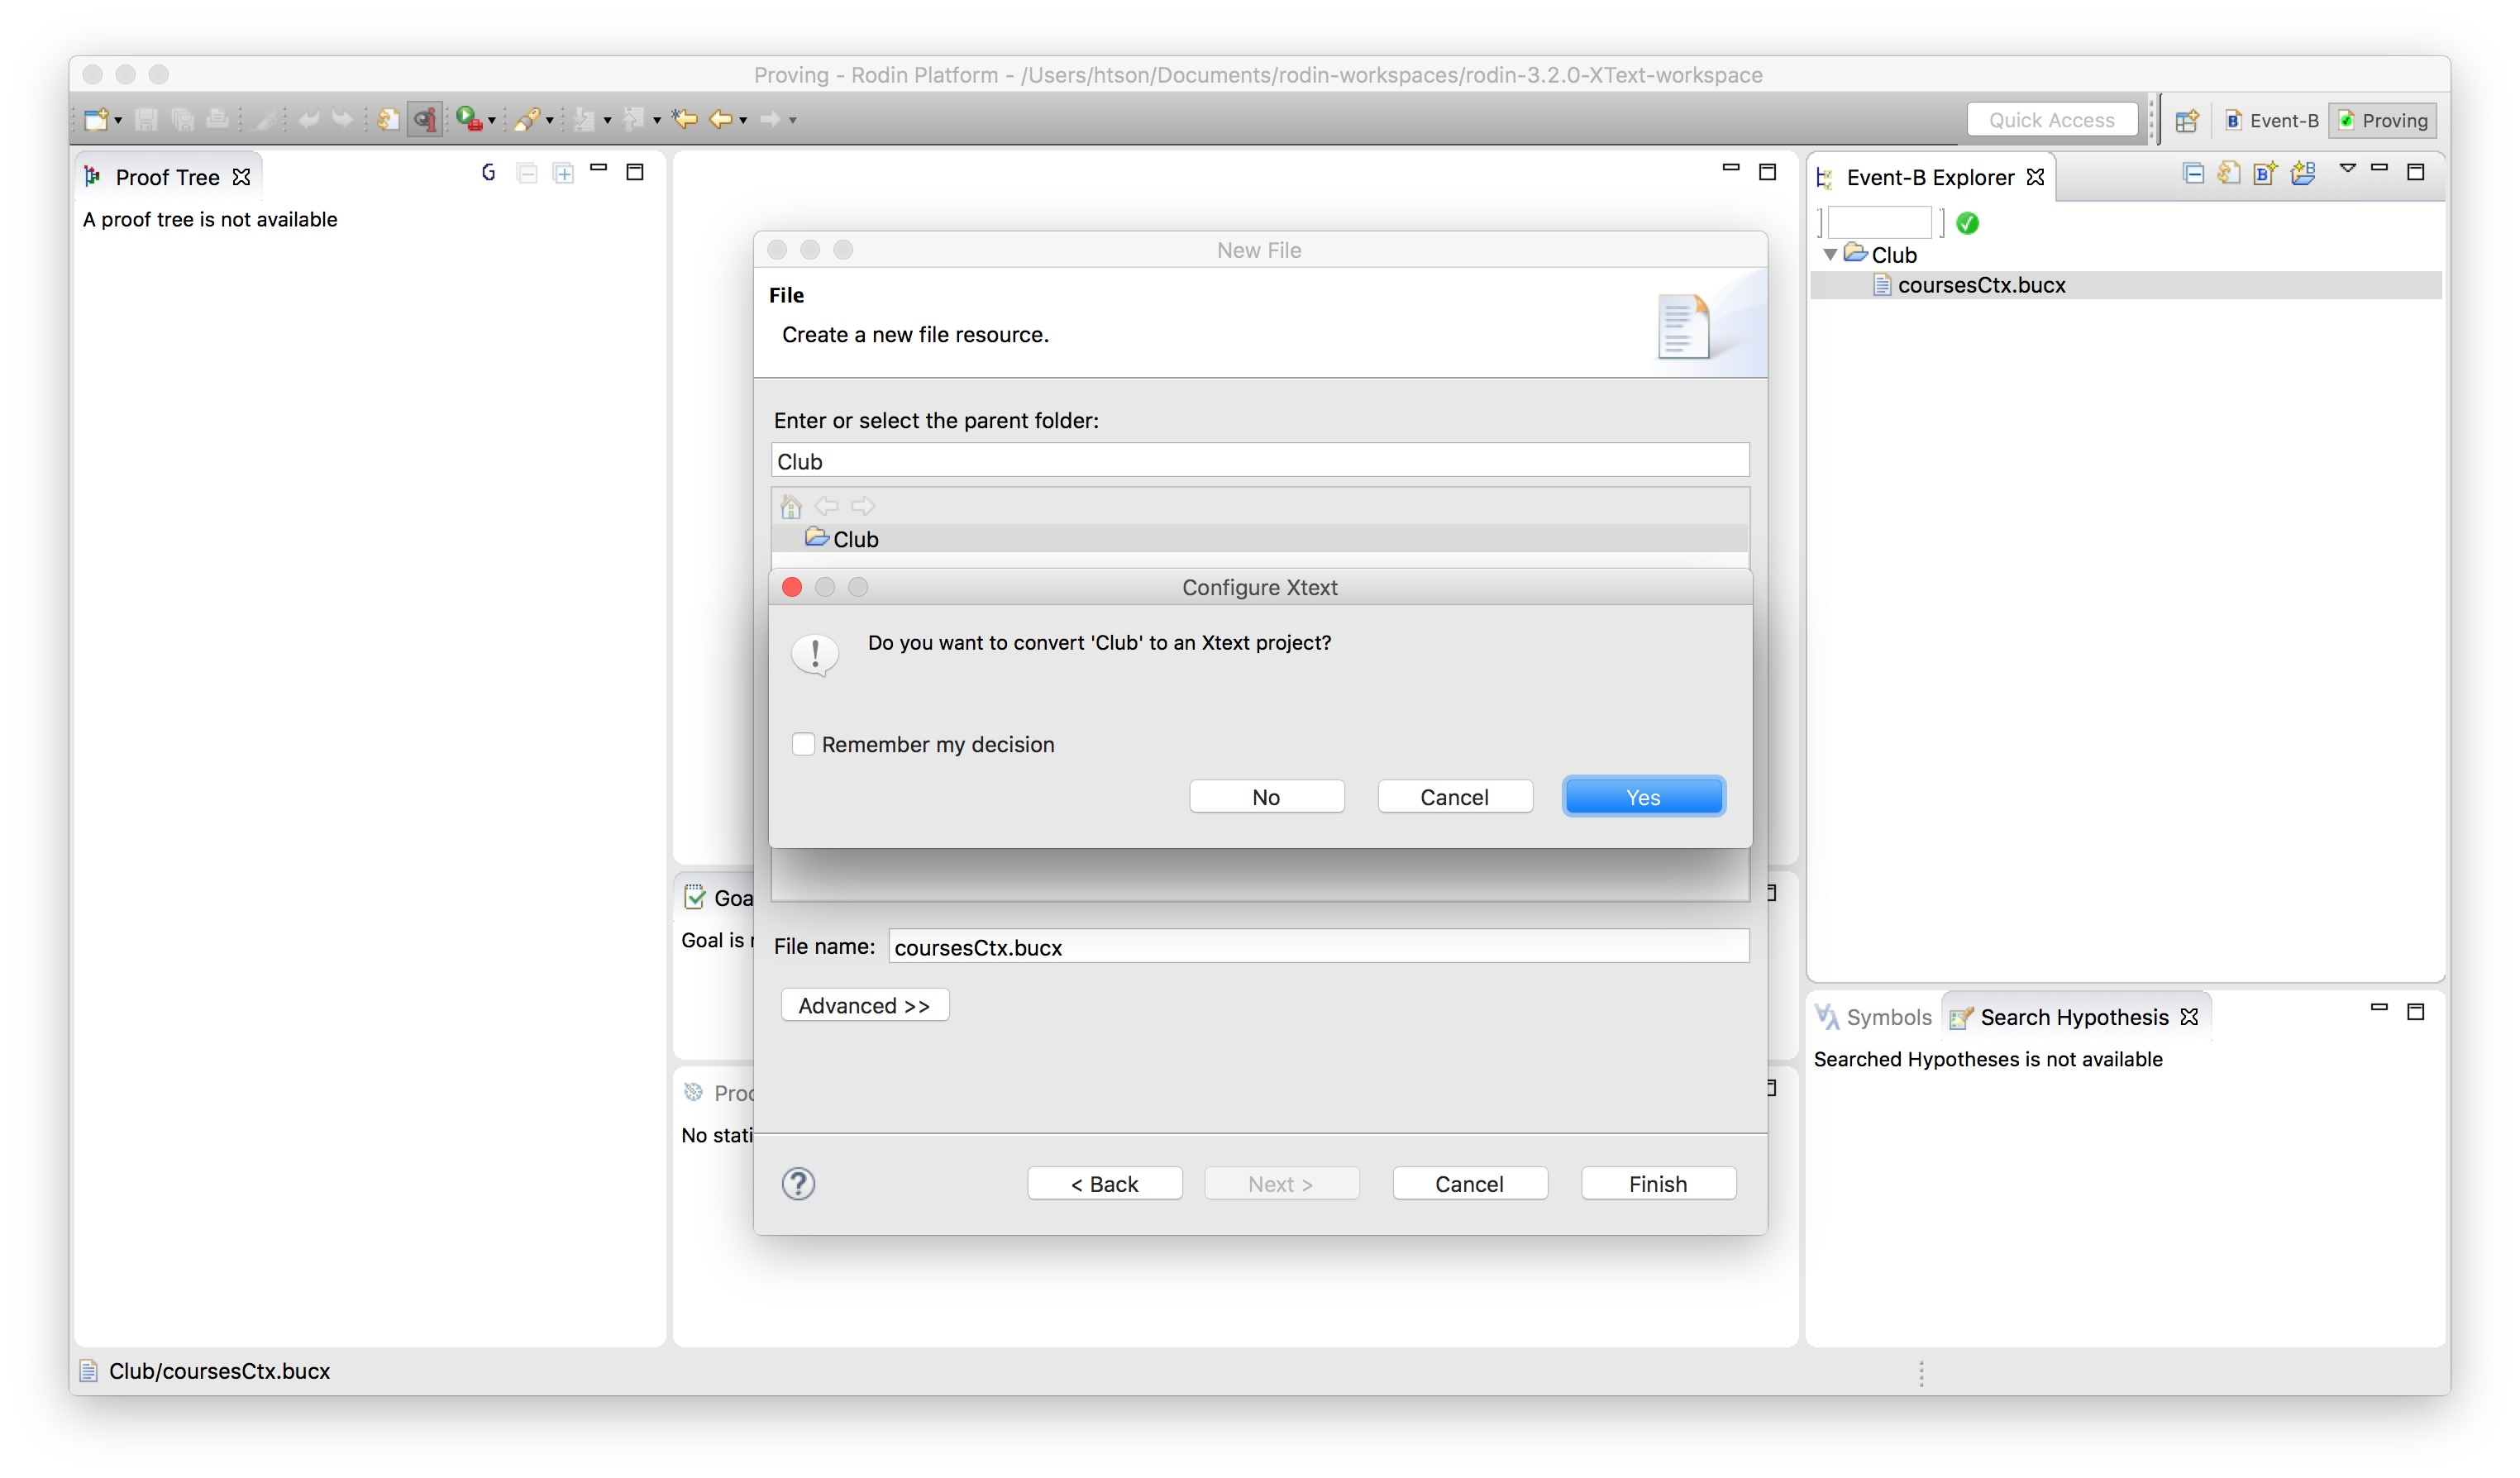
\includegraphics[width=512]{figures/ConvertToXText}
  \else
  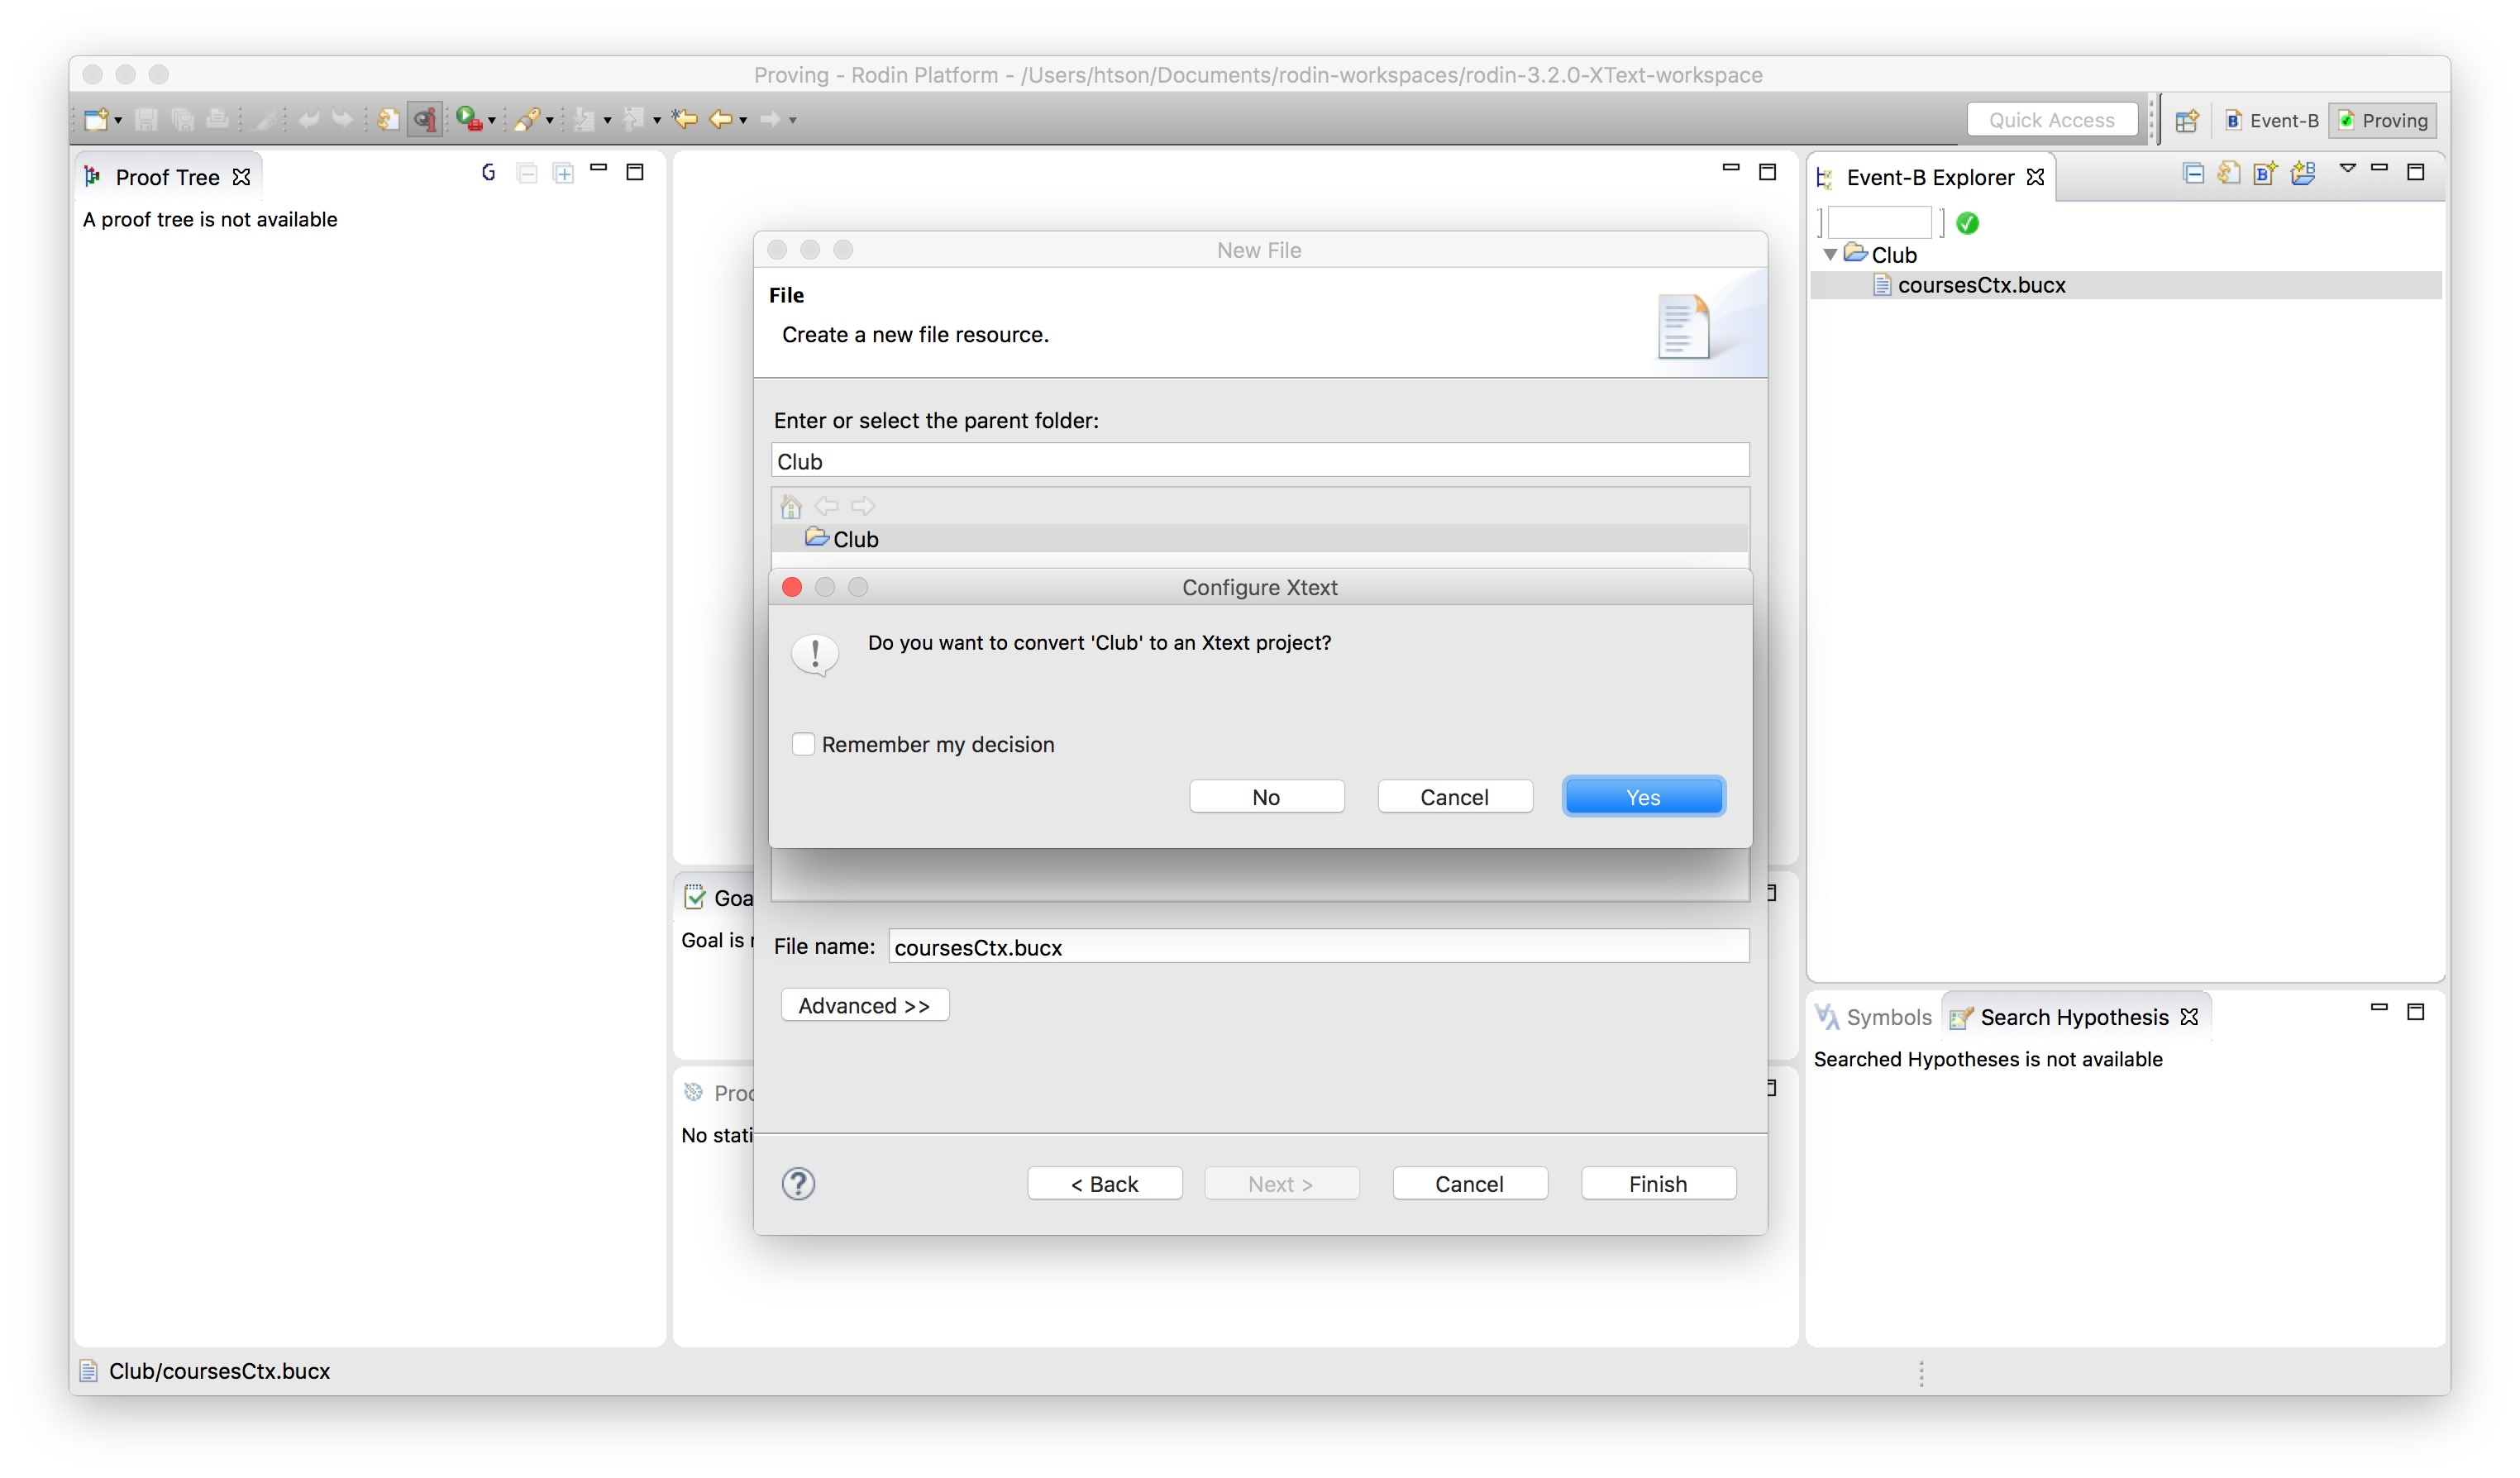
\includegraphics[width=0.9\textwidth]{figures/ConvertToXText}
  \fi
  \caption{Convert ``Club'' to XText project}
  \label{fig:ConvertToXText}
\end{figure}

\item[Step 2. Set the content of courseCtx.bucx] Set the content of ``coursesCtx.bucx'' as follows.
  \begin{center}
    \begin{Bcode}
      \ifplastex
      \Bcontext{} coursesCtx\\
      \Bsets{} CRS\\
      \Bconstants{} m\\
      \Baxioms\\
      @axm0_1: "finite(CRS)"\\
      @axm0_2: "m ∈ ℕ1"\\
      @thm0_1: "0 < m" \Btheorem\\
      \Bend
      \else
\Bcontext{} coursesCtx\\
\Bsets{} CRS\\
\Bconstants{} m\\
\Baxioms\\
\Btab @axm0\_1: "\(\finite(CRS)\)"\\
\Btab @axm0\_2: "\(m \in \natn\)"\\
\Btab @thm0\_1: "\(0 < m\)" \Btheorem\\
\Bend
       \fi
    \end{Bcode}
  \end{center}

\item[Step 3. Auto-format the code] Automatically format the content of ``coursesCtx.bucx'' using short-cut (e.g., on Mac OS: \texttt{Cmd+Shift+F}).

\item[Step 4. Save the file] \textbf{Save the file ``coursesCtx.bucx''}.
\end{description}
\textbf{Conclusion} By now, the XContext ``coursesCtx.bucx'' and the corresponding Rodin Context ``coursesCtx'' should be visible in the Event-B Explorer.
\begin{description}
\item[Step 1. Create a new XMachine m0.bumx] Create a new XMachine named ``m0.bumx'' using the \emph{New File wizard}. The newly created file should be opened automatically in an XMachine editor.
\end{description}

\textbf{Conclusion} By now, the XMachine ``m0.bumx'' and the corresponding Rodin Machine ``m0'' (without any error) should be visible in the Event-B Explorer.

\subsubsection{Task 4. Create a simple XMachine m0.bumx}
\textbf{Introduction} The purpose of this task is to create a simple XMachine within the newly created project.

\begin{description}
\item[Step 1. Create a new XMachine m0.bumx] \textbf{Create a new XMachine} named ``m0.bumx'' using the New File wizard. The newly created file should be opened automatically in an XMachine editor.

\item[Step 2. Set the content of m0.bumx] \textbf{Set the content of "m0.bumx" as follows}.
  \begin{center}
    \begin{Bcode}
      \ifplastex
      \Bmachine{} m0 \\
      \Bvariables{} crs \\
      \Binvariants \\
      @inv0_1: "crs ∈ ℙ(CRS)"\\
      @thm0_2: "finite(crs)" \Btheorem \\
      @inv0_2: "card(crs) ≤ m" \\
      @DLF: "(card(crs) ≠ m) ∨ (∃cs·cs ⊆ crs ∧ cs ≠ ∅)" \\
      \Bevents\\
      INITIALISATION\\
      \Bbegin \\
      @act0_1: "crs ≔ ∅"\\
      \Bend\\
      OpenCourses\\
      \Bwhen\\
      @grd0_1: "card(crs) ≠ m" \\
      @thm0_3: "crs ≠ CRS" \Btheorem \\
      \Bthen\\
      @act0_1: "crs :∣ crs ⊂ crs' ∧ card(crs') ≤ m"\\
      \Bend\\
      CloseCourses \Banticipated\\
      \Bany{} cs \Bwhere\\
      @grd0_1: "cs ⊆ crs"\\
      @grd0_2: "cs ≠ ∅"\\
      \Bthen\\
      @act0_1: "crs ≔ crs ∖ cs"\\
      \Bend\\
      \Bend
      \else
      \Bmachine{} m0 \\
      \Bvariables{} crs \\
      \Binvariants \\
      \Btab @inv0\_1: "\(crs \in \pow(CRS)\)"\\
      \Btab @thm0\_2: "\(\finite(crs)\)" \Btheorem \\
      \Btab @inv0\_2: "\(\card(crs) \leq m\)" \\
      \Btab @DLF: "\((\card(crs) \neq m) \lor (\exists cs \qdot cs \subseteq crs \land cs \neq \emptyset)\)" \\
      \Bevents\\
      \Btab INITIALISATION\\
      \Btab \Bbegin \\
      \Btab\Btab @act0\_1: "\(crs \bcmeq \emptyset\)"\\
      \Btab \Bend\\
      \Btab OpenCourses\\
      \Btab \Bwhen\\
      \Btab \Btab @grd0\_1: "\(\card(crs) \neq m\)" \\
      \Btab \Btab @thm0\_3: "\(crs \neq CRS\)" \Btheorem \\
      \Btab \Bthen\\
      \Btab \Btab @act0\_1: "\(crs \bcmsuch crs \subset crs' \land \card(crs') \leq m\)"\\
      \Btab \Bend\\
      \Btab CloseCourses \Banticipated\\
      \Btab \Bany{} cs \Bwhere\\
      \Btab \Btab @grd0\_1: "\(cs \leq crs\)"\\
      \Btab \Btab @grd0\_2: "\(cs \neq \emptyset\)"\\
      \Btab \Bthen\\
      \Btab \Btab @act0\_1: "\(crs \bcmeq crs \setminus cs\)"\\
      \Btab \Bend\\
      \Bend
      \fi
    \end{Bcode}
  \end{center}
\item[Step 3. Auto-format the code] \textbf{Automatically format the content of ``m0.bumx''} by using short-cut (e.g., on Mac OS: Cmd+Shift+F).

\item[Step 4. Save the file] \textbf{Save the file ``m0.bumx''}.

\item[Step 5. Add missing ``sees'' clause] In the compiled Rodin Machine m0, there are several errors, due to the fact that \textbf{m0} refers to the sets and constants of the context courseCtx.
  \textbf{Add the missing ``sees'' clause} after the ``machine'' clause
  \begin{center}
    \begin{Bcode}
      \Bsees{} courseCtx
    \end{Bcode}
  \end{center}
  (Note: One can use \emph{Content Assist} after typing the ``sees'' keyword to select the context.
  
\item[Step 6. Save the file again] \textbf{Save the file "m0.bumx" again}.
\end{description}
\textbf{Conclusion} By now, the XMachine ``m0.bumx'' and the corresponding Rodin Machine ``m0'' (without any error) should be visible in the Event-B Explorer.

\subsubsection{Task 5. Create extended XContexts}
\textbf{Introduction} The purpose of this task is to create some more extended XContexts within the "Club" project.

\paragraph{Task 5.1. Create a simple XContext membersCtx.bucx}
\textbf{Introduction} The purpose of this sub-task is to create a simple XContext ``membersCtx.bucx'' within the ``Club'' project.
\begin{description}
\item[Step 1. Create a new XContext membersCtx.bucx] \textbf{Create a new XContext} named ``membersCtx.bucx'' using the \emph{New File} wizard.

\item[Step 2. Set the content of courseCtx.bucx] \textbf{Set the content of ``membersCtx.bucx'' as follows}.
  \begin{center}
    \begin{Bcode}
      \ifplastex
      \Bcontext{} memebersCtx\\
      \Bsets{} MEM\\
      \Baxioms\\
      @axm0_1: "finite(MEM)"\\
      \Bend
      \else
      \Bcontext{} memebersCtx\\
      \Bsets{} MEM\\
      \Baxioms\\
      \Btab @axm0_1: "\(\finite(MEM)\)"\\
      \Bend
      \fi
    \end{Bcode}
  \end{center}

\item [Step 3. Auto-format the code] \textbf{Automatically format the content of ``membersCtx.bucx''} by using short-cut (e.g., on Mac OS: Cmd+Shift+F).

\item[Step 4. Save the file] <b>Save the file \textbf{``membersCtx.bucx''}.
\end{description}

\textbf{Conclusion} By now, the XContext ``membersCtx.bucx'' and the corresponding Rodin Context ``membersCtx'' should be visible in the Event-B Explorer.

\paragraph{Task 5.2. Create an extended XContext participantsCtx.bucx}
\textbf{Introduction} The purpose of this sub-task is to create an extended XContext ``participantsCtx.bucx'' within the ``Club'' project.

\begin{description}
\item[Step 1. Create a new XContext participantsCtx.bucx] \textbf{Create a new XContext} named ``participantsCtx.bucx'' using the \emph{New File wizard}.

\item[Step 2. Set the content of participantsCtx.bucx] \textbf{Set the content of ``participantsCtx.bucx'' as follows}.
  \begin{center}
    \begin{Bcode}
      \ifplastex
      \Bcontext{} participantsCtx\\
      \Bextends{} membersCtx\\
      \Bconstants{} PRTCPT\\
      \Baxioms\\
      @axm1_2: "PRTCPT ∈ ℙ(MEM)"\\
      @thm1_1: "finite(PRTCPT)" \Btheorem\\
      \Bend
      \else
      \Bcontext{} participantsCtx\\
      \Bextends{} membersCtx\\
      \Bconstants{} PRTCPT\\
      \Baxioms\\
      \Btab @axm1_2: "\(PRTCPT \in \pow(MEM)\)"\\
      \Btab @thm1_1: "\(\finite(PRTCPT)\)" \Btheorem\\
      \Bend
      \fi
    \end{Bcode}
  \end{center}

\item[Step 3. Auto-format the code] \textbf{Automatically format the content of ``participantsCtx.bucx''} by using short-cut (e.g., on Mac OS: Cmd+Shift+F).

\item[Step 4. Save the file] \textbf{Save the file ``participantsCtx.bucx''}.
\end{description}

\textbf{Conclusion} By now, the XContext ``participantsCtx.bucx'' and the corresponding Rodin Context ``participantsCtx'' should be visible in the Event-B Explorer.

\paragraph{Task 5.3. Create an extended XContext instructorsCtx.bucx}
\textbf{Introduction} The purpose of this sub-task is to create an extended XContext ``instructorsCtx.bucx'' within the ``Club'' project.
\begin{description}
\item[Step 1. Create a new XContext instructorsCtx.bucx] \textbf{Create a new XContext} named ``instructorsCtx.bucx'' using the \emph{New File wizard}.

\item[Step 2. Set the content of instructorsCtx.bucx] \textbf{Set the content of ``instructorsCtx.bucx'' as follows}.
  \begin{center}
    \begin{Bcode}
      \ifplastex
      \Bcontext{} instructorsCtx\\
      \Bextends{} membersCtx coursesCtx\\
      \Bconstants{} INSTR instrs\\
      \Baxioms\\
      @axm1_3: "INSTR ∈ ℙ(MEM)"\\
      @axm1_4: "instrs ∈ CRS → INSTR"\\
      \Bend
      \else
      \Bcontext{} instructorsCtx\\
      \Bextends{} membersCtx coursesCtx\\
      \Bconstants{} INSTR instrs\\
      \Baxioms\\
      \Btab @axm1_3: "\(INSTR \in \pow(MEM)\)"\\
      \Btab @axm1_4: "\(instrs \in CRS \tfun INSTR\)"\\
      \Bend
      \fi
    \end{Bcode}
  \end{center}

\item[Step 3. Auto-format the code] \textbf{Automatically format the content of ``intructorsCtx.bucx''} by using short-cut (e.g., on Mac OS: Cmd+Shift+F).

\item[Step 4. Save the file] \textbf{Save the file ``instructorsCtx.bucx''}.
\end{description}

\textbf{Conclusion} By now, the XContext ``instructorsCtx.bucx'' and the corresponding Rodin Context ``instructorsCtx'' should be visible in the Event-B Explorer.

\subsubsection{Task 6. Create refined XMachines}
\textbf{Introduction} The purpose of this task is to create some more refined XMachines within the ``Club'' project.

\paragraph{Task 6.1. Create a refined XMachine m1.bumx}
\textbf{Introduction} The purpose of this sub-task is to create a refined XMachine ``m1.bumx'' within the ``Club'' project.
\begin{description}
\item[Step 1. Create a new XMachine m1.bumx] \textbf{Create a new XMachine} named ``m1.bumx'' using the \emph{New File wizard}. The newly created file should be opened automatically in an XMachine editor.

\item[Step 2. Set the content of m1.bumx] \textbf{Set the content of ``m1.bumx'' as follows}.
  \begin{center}
    \begin{Bcode}
      \ifplastex
      \Bmachine{} m1\\
      \Brefines{} m0\\
      \Bsees{} instructorsCtx participantsCtx \\
      \Bvariables{} crs prtcpts \\
      \Binvariants\\
      @inv1_1: "prtcpts ∈ crs ↔ PRTCPT"\\
      @inv1_2: "∀c·c ∈ crs ⇒ instrs(c) ∉ prtcpts[{c}]"\\
      \Bvariant{} "(crs × PRTCPT) ∖ prtcpts"\\
      \Bevents\\
      INITIALISATION \Bextended\\
      \Bbegin\\
      @act1_2: "prtcpts ≔ ∅"\\
      \Bend\\
      OpenCourses \Bextended\\
      \Brefines{} OpenCourses\\
      \Bwhen\\
      @thm1_2: "dom(prtcpts) ⊆ crs" theorem \\
      \Bend\\
      CloseCourses \Bextended{} \Banticipated\\
      \Brefines{} CloseCourses\\
      \Bbegin\\
      @act1_2: "prtcpts ≔ cs ⩤ prtcpts"\\
      \Bend\\
      Register \Bconvergent\\
      \Bany{} p c \Bwhere \\
      @grd1_1: "p ∈ PRTCPT"\\
      @grd1_2: "c ∈ crs"\\
      @grd1_3: "p ≠ instrs(c)"\\
      @grd1_4: "c ↦ p ∉ prtcpts"\\
      \Bthen\\
      @act1_1: "prtcpts ≔ prtcpts ∪ {c ↦ p}"\\
      \Bend\\
      \Bend
      \else
      \Bmachine{} m1\\
      \Brefines{} m0\\
      \Bsees{} instructorsCtx participantsCtx \\
      \Bvariables{} crs prtcpts \\
      \Binvariants\\
      \Btab @inv1_1: "\(prtcpts \in crs \rel PRTCPT\)"\\
      \Btab @inv1_2: "\(\forall c \qdot c ∈ crs \limp instrs(c) \notin prtcpts[\{c\}]\)"\\
      \Bvariant{} "\((crs \cprod PRTCPT) \setminus prtcpts\)"\\
      \Bevents\\
      \Btab INITIALISATION \Bextended\\
      \Btab \Bbegin\\
      \Btab \Btab @act1_2: "\(prtcpts \bcmeq \emptyset\)"\\
      \Btab \Bend\\
      \Btab OpenCourses \Bextended\\
      \Btab \Brefines{} OpenCourses\\
      \Btab \Bwhen\\
      \Btab \Btab @thm1_2: "\(\dom(prtcpts) \subseteq crs\)" theorem \\
      \Btab \Bend\\
      \Btab CloseCourses \Bextended{} \Banticipated\\
      \Btab \Brefines{} CloseCourses\\
      \Btab \Bbegin\\
      \Btab \Btab @act1_2: "\(prtcpts \bcmeq cs \domsub prtcpts\)"\\
      \Btab \Bend\\
      \Btab Register \Bconvergent\\
      \Btab \Bany{} p c \Bwhere \\
      \Btab \Btab @grd1_1: "\(p \in PRTCPT\)"\\
      \Btab \Btab @grd1_2: "\(c \in crs\)"\\
      \Btab \Btab @grd1_3: "\(p \neq instrs(c)\)"\\
      \Btab \Btab @grd1_4: "\(c \mapsto p \neq prtcpts\)"\\
      \Btab \Bthen\\
      \Btab \Btab @act1_1: "\(prtcpts \bcmeq prtcpts \bunion \{c \mapsto p\}\)"\\
      \Btab \Bend\\
      \Bend
      \fi
    \end{Bcode}
  \end{center}

\item[Step 3. Auto-format the code] \textbf{Automatically format the content of ``m1.bumx''} by using short-cut (e.g., on Mac OS: Cmd+Shift+F).

\item[Step 4. Save the file] Save the file ``m1.bumx''.
\end{description}

\textbf{Conclusion} By now, the XMachine ``m1.bucx'' and the corresponding Rodin Machine ``m1'' should be visible in the Event-B Explorer.

\paragraph{Task 6.2. Create a refined XMachine m2.bumx}
\textbf{Introduction} The purpose of this sub-task is to create a refined XMachine ``m2.bumx'' within the ``Club'' project.

\begin{description}
\item[Step 1. Create a new XMachine m2.bumx] \textbf{Create a new XMachine} named ``m2.bumx'' using the \emph{New File wizard}. The newly created file should be opened automatically in an XMachine editor.

\item[Step 2. Set the content of m2.bumx] \textbf{Set the content of ``m2.bumx'' as follows}.
  \begin{center}
    \begin{Bcode}
      \ifplastex
      \Bmachine{} m2\\
      \Brefines{} m1\\
      \Bsees{} instructorsCtx participantsCtx\\
      \Bvariables{} atnds\\
      \Binvariants\\
      @inv2_1: "atnds ∈ CRS ⇸ ℙ(PRTCPT)"\\
      @inv2_2: "crs = dom(atnds)"\\
      @inv2_3: "∀c·c ∈ crs ⇒ prtcpts[{c}] = atnds(c)"\\
      @thm2_1: "finite(atnds)" \Btheorem\\
      \Bvariant{} "card(atnds)"\\
      \Bevents\\
      INITIALISATION\\
      \Bbegin\\
      @act2_1: "atnds ≔ ∅"\\
      \Bend\\
      OpenCourse\\
      \Brefines{} OpenCourses\\
      \Bany{} c \Bwhere\\
      @grd2_1: "c ∉ dom(atnds)"\\
      @grd2_2: "card(atnds) ≠ m" \\
      @thm2_2: "card(crs) ≠ m" theorem\\
      \Bwith\\
      @crs': "crs' = crs ∪ {c}"\\
      \Bthen\\
      @act2_1: "atnds(c) ≔ ∅"\\
      \Bend\\
      CloseCourse \Bconvergent\\
      \Brefines{} CloseCourses\\
      \Bany{} c \Bwhere\\
      @grd2_1: "c ∈ dom(atnds)"\\
      \Bwith\\
      @cs: "cs = {c}"\\
      \Bthen\\
      @act1_2: "atnds ≔ {c} ⩤ atnds"\\
      \Bend\\
      Register \Bconvergent\\
      \Brefines Register\\
      \Bany{} p c \Bwhere\\
      @grd2_1: "p ∈ PRTCPT"\\
      @grd2_2: "p ≠ instrs(c)"\\
      @grd2_3: "c ∈ dom(atnds)"\\
      @grd2_4: "p ∉ atnds(c)"\\
      @thm2_3: "atnds(c) = prtcpts[{c}]" theorem\\
      \Bthen\\
      @act2_1: "atnds(c) ≔ atnds(c) ∪ {p}"\\
      \Bend\\
      \Bend
      \else
      \Bmachine{} m2\\
      \Brefines{} m1\\
      \Bsees{} instructorsCtx participantsCtx\\
      \Bvariables{} atnds\\
      \Binvariants\\
      \Btab @inv2_1: "\(atnds \in CRS \pfun \pow(PRTCPT)\)"\\
      \Btab @inv2_2: "\(crs = \dom(atnds)\)"\\
      \Btab @inv2_3: "\(\forall c \qdot c \in crs \limp prtcpts[\{c\}] = atnds(c)\)"\\
      \Btab @thm2_1: "\(\finite(atnds)\)" \Btheorem\\
      \Bvariant{} "\(\card(atnds)\)"\\
      \Bevents\\
      \Btab INITIALISATION\\
      \Btab \Bbegin\\
      \Btab \Btab @act2_1: "\(atnds \bcmeq \emptyset\)"\\
      \Btab \Bend\\
      \Btab OpenCourse\\
      \Btab \Brefines{} OpenCourses\\
      \Btab \Bany{} c \Bwhere\\
      \Btab \Btab @grd2_1: "\(c \notin \dom(atnds)\)"\\
      \Btab \Btab @grd2_2: "\(\card(atnds) \neq m\)" \\
      \Btab \Btab @thm2_2: "\(\card(crs) \neq m\)" \Btheorem\\
      \Btab \Bwith\\
      \Btab \Btab @crs': "\(crs' = crs \bunion \{c\}\)"\\
      \Btab \Bthen\\
      \Btab \Btab @act2_1: "\(atnds(c) \bcmeq \emptyset\)"\\
      \Btab \Bend\\
      \Btab CloseCourse \Bconvergent\\
      \Btab \Brefines{} CloseCourses\\
      \Btab \Bany{} c \Bwhere\\
      \Btab \Btab @grd2_1: "\(c \in \dom(atnds)\)"\\
      \Btab \Bwith\\
      \Btab \Btab @cs: "\(cs = \{c\}\)"\\
      \Btab \Bthen\\
      \Btab \Btab @act1_2: "\(atnds \bcmeq \{c\} \domsub atnds\)"\\
      \Btab \Bend\\
      \Btab  Register \Bconvergent\\
      \Btab \Brefines Register\\
      \Btab \Bany{} p c \Bwhere\\
      \Btab \Btab @grd2_1: "\(p \in PRTCPT\)"\\
      \Btab \Btab @grd2_2: "\(p \neq instrs(c)\)"\\
      \Btab \Btab @grd2_3: "\(c \in \dom(atnds)\)"\\
      \Btab \Btab @grd2_4: "\(p \notin atnds(c)\)"\\
      \Btab \Btab @thm2_3: "\(atnds(c) = prtcpts[\{c\}]\)" theorem\\
      \Btab \Bthen\\
      \Btab \Btab @act2_1: "\(atnds(c) \bcmeq atnds(c) ∪ \{p\}\)"\\
      \Btab \Bend\\
      \Bend
      \fi
    \end{Bcode}
  \end{center}
\end{description}
\textbf{Conclusion} By now, the XMachine ``m2.bucx'' and the corresponding Rodin Machine ``m2'' should be visible in the Event-B Explorer.

%%% Local Variables:
%%% mode: latex
%%% TeX-master: "user_manual"
%%% End:
